\documentclass[aspectratio=169, 11pt]{beamer}

% --- Theme & Colors ---
\usetheme{metropolis}
\usepackage{appendixnumberbeamer}
\usepackage{booktabs}
\usepackage{graphicx}
\usepackage{xcolor}
\usepackage{tikz}
\usetikzlibrary{shapes, arrows.meta, positioning, calc, decorations.pathreplacing}
\usepackage{fontawesome5}
\usepackage{multicol}
\usepackage{adjustbox}

% Custom colors
\definecolor{UMNMaroon}{HTML}{7A0019}
\definecolor{UMNGold}{HTML}{FFCC33}
\definecolor{DarkBlue}{HTML}{1a237e}
\definecolor{AccentGreen}{HTML}{2e7d32}
\definecolor{AccentOrange}{HTML}{e65100}
\definecolor{LightGray}{HTML}{f5f5f5}
\definecolor{PhaseBlue}{HTML}{1565c0}
\definecolor{PhaseGreen}{HTML}{2e7d32}
\definecolor{PhaseOrange}{HTML}{ef6c00}
\definecolor{PhasePurple}{HTML}{6a1b9a}
\definecolor{PhaseRed}{HTML}{c62828}
\definecolor{PhaseTeal}{HTML}{00838f}

\setbeamercolor{frametitle}{bg=UMNMaroon, fg=white}
\setbeamercolor{progress bar}{fg=UMNGold}
\setbeamercolor{title separator}{fg=UMNGold}
\setbeamercolor{alerted text}{fg=AccentOrange}

% Figure path
\graphicspath{{../figures/}}

% Compact itemize
\setlength{\leftmargini}{1.2em}
\setlength{\leftmarginii}{1.0em}

% Tighter list spacing
\setbeamertemplate{itemize/enumerate body begin}{\small}
\setbeamertemplate{itemize/enumerate subbody begin}{\footnotesize}

% --- Title ---
\title{E-Scooter Speed Safety in South Korea}
\subtitle{Project Progress: From Raw GPS to Submission-Ready Manuscript}
\author{Seongjin Choi}
\institute{University of Minnesota Twin Cities\\Department of Civil, Environmental, and Geo- Engineering}
\date{March 2026}

\begin{document}

% ============================================================
% TITLE
% ============================================================
\begin{frame}[plain,noframenumbering]
\maketitle
\end{frame}

% ============================================================
% OUTLINE
% ============================================================
\begin{frame}{Presentation Outline}
\begin{columns}[T]
\begin{column}{0.48\textwidth}
\textbf{Part I --- Data \& Exploration}
\begin{enumerate}
\item Project Motivation
\item Data Preprocessing (Phase 1)
\item Speed Indicators (Phase 2)
\item Map-Matching \& Road Class (Phase 3)
\item Spatial Analysis (Phase 4)
\end{enumerate}
\end{column}
\begin{column}{0.48\textwidth}
\textbf{Part II --- Modeling \& Paper}
\begin{enumerate}\setcounter{enumi}{5}
\item Statistical Modeling (Phase 5)
\item Extension Analyses (Phase 8)
\item DiD Causal Analysis (Phase 11)
\item Survival Analysis (Phase 12)
\item Paper Status \& Next Steps
\end{enumerate}
\end{column}
\end{columns}
\vfill
\footnotesize Target venue: \textit{Transportation Research Part C} \hfill 101/107 tasks complete
\end{frame}

% ============================================================
% 1. MOTIVATION
% ============================================================
\section{Project Motivation}

\begin{frame}{Why E-Scooter Speed Safety?}
\begin{columns}[T]
\begin{column}{0.55\textwidth}
\textbf{Context}
\begin{itemize}
\item E-scooters: fastest-growing micro-mobility mode
\item South Korea: 25 km/h speed limit
\item Swing: largest Korean operator
\item Modes: \textbf{TUB} (turbo), \textbf{STD}, \textbf{ECO}
\end{itemize}
\vspace{0.15cm}
\textbf{Research Gaps}
\begin{itemize}
\item No large-scale GPS study for e-scooter speeding
\item Mode-specific speed governance poorly understood
\item Causal evidence on speed limiters missing
\end{itemize}
\end{column}
\begin{column}{0.43\textwidth}
\centering
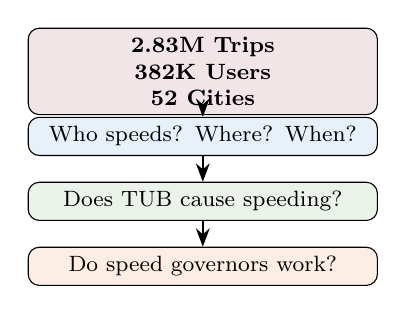
\begin{tikzpicture}[scale=0.75]
\node[draw, rounded corners, fill=UMNMaroon!10, text width=4.2cm, align=center, font=\footnotesize\bfseries] (data) at (0,3.6) {2.83M Trips\\382K Users\\52 Cities};
\node[draw, rounded corners, fill=PhaseBlue!10, text width=4.2cm, align=center, font=\footnotesize] (q1) at (0,2.5) {Who speeds? Where? When?};
\node[draw, rounded corners, fill=AccentGreen!10, text width=4.2cm, align=center, font=\footnotesize] (q2) at (0,1.4) {Does TUB cause speeding?};
\node[draw, rounded corners, fill=AccentOrange!10, text width=4.2cm, align=center, font=\footnotesize] (q3) at (0,0.3) {Do speed governors work?};
\draw[-{Stealth}, thick] (data) -- (q1);
\draw[-{Stealth}, thick] (q1) -- (q2);
\draw[-{Stealth}, thick] (q2) -- (q3);
\end{tikzpicture}
\end{column}
\end{columns}
\end{frame}

\begin{frame}{Dataset Overview}
\begin{columns}[T]
\begin{column}{0.45\textwidth}
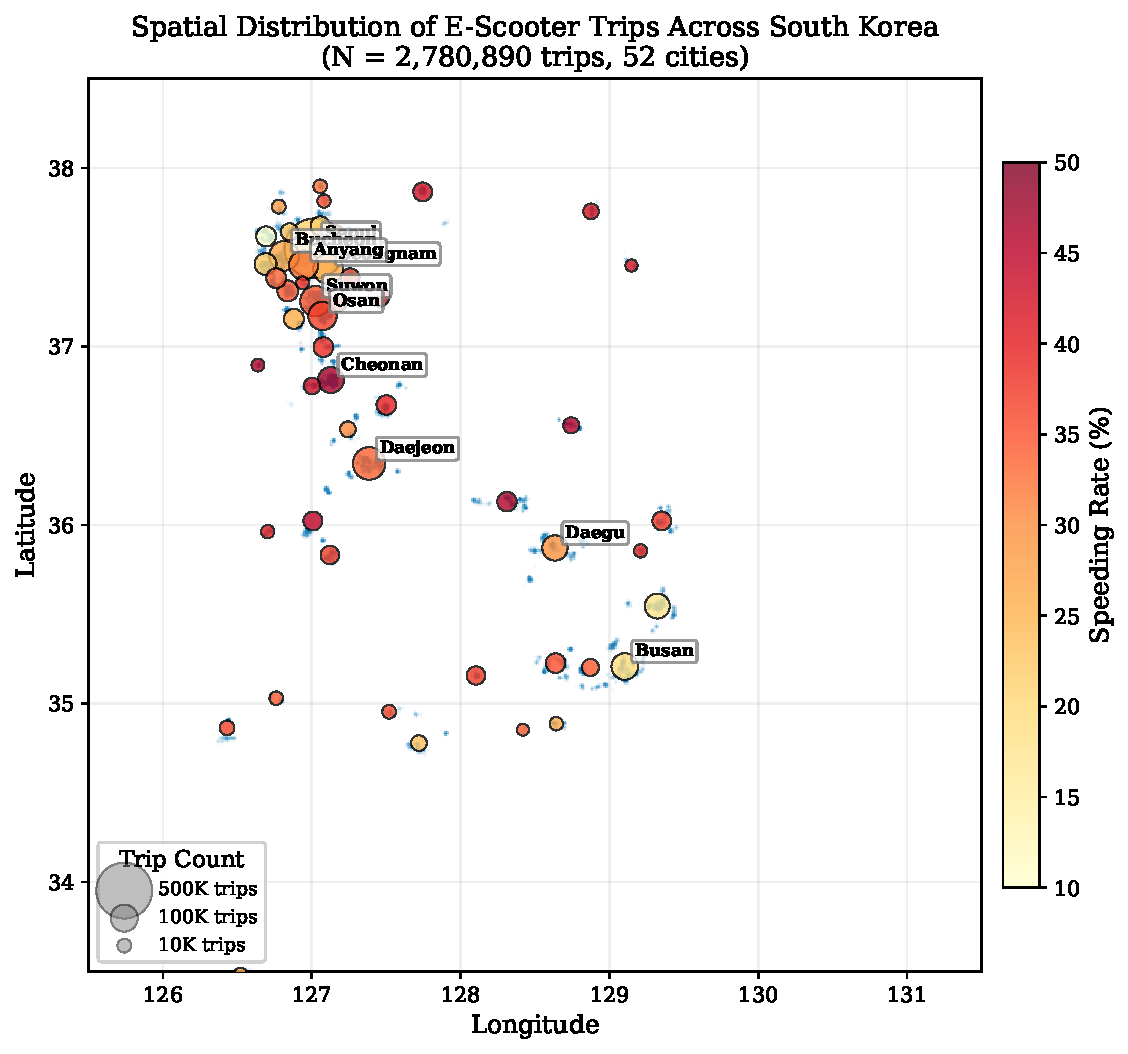
\includegraphics[width=\textwidth]{fig1_spatial_distribution.pdf}
\end{column}
\begin{column}{0.52\textwidth}
\textbf{Swing GPS Trajectories}
\begin{itemize}
\item \textbf{Cross-section}: 2.83M trips (May 2023)
\item \textbf{Longitudinal}: 44.1M trips (24 months)
\item Speed data: Feb--Dec 2023 only
\item 25 columns: GPS, speeds, mode, model
\end{itemize}
\vspace{0.15cm}
\textbf{Key characteristics}
\begin{itemize}
\item Sensor-based speeds (not GPS-derived)
\item GPS interval $\sim$10s; sentinel $-999$ for NULL
\item 17 provinces, 52 cities
\end{itemize}
\end{column}
\end{columns}
\end{frame}

% ============================================================
% 2. PHASE 1: DATA PREPROCESSING
% ============================================================
\section{Phase 1: Data Preprocessing}

\begin{frame}{Phase 1: Data Quality Control}
\textbf{Why}: Raw GPS data contains errors and inconsistencies that would bias all downstream analyses.

\begin{columns}[T]
\begin{column}{0.52\textwidth}
\textbf{Pipeline (7 tasks)}
\begin{enumerate}
\item Profile schema: null rates, types, ranges
\item Filter: I9 outliers ($>$50 km/h), zero-distance, $<$5 GPS points
\item City assignment: KD-tree to 54 city centers
\item Per-city summary statistics
\item Validate \texttt{speeds} vs.\ displacement-derived
\item Build cleaned Parquet dataset
\item Data quality report
\end{enumerate}
\end{column}
\begin{column}{0.45\textwidth}
\centering
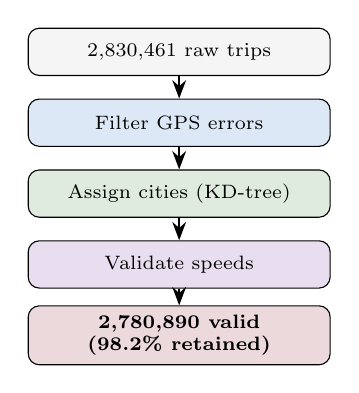
\begin{tikzpicture}[
  box/.style={draw, rounded corners, fill=#1, text width=3.6cm, align=center, minimum height=0.6cm, font=\scriptsize},
  arr/.style={-{Stealth}, thick}
]
\node[box=LightGray] (raw) at (0,3.6) {2,830,461 raw trips};
\node[box=PhaseBlue!15] (filter) at (0,2.7) {Filter GPS errors};
\node[box=PhaseGreen!15] (city) at (0,1.8) {Assign cities (KD-tree)};
\node[box=PhasePurple!15] (valid) at (0,0.9) {Validate speeds};
\node[box=UMNMaroon!15, font=\scriptsize\bfseries] (clean) at (0,0) {2,780,890 valid\\(98.2\% retained)};
\draw[arr] (raw) -- (filter);
\draw[arr] (filter) -- (city);
\draw[arr] (city) -- (valid);
\draw[arr] (valid) -- (clean);
\end{tikzpicture}
\end{column}
\end{columns}
\end{frame}

% ============================================================
% 3. PHASE 2: SPEED INDICATORS
% ============================================================
\section{Phase 2: Speed Indicators}

\begin{frame}{Phase 2: Computing Speed Safety Indicators}
\textbf{Why}: Transform raw speed arrays into interpretable metrics for modeling.

\begin{columns}[T]
\begin{column}{0.50\textwidth}
\textbf{Trip-level indicators}
\begin{itemize}
\item Mean/max/P85 speed, speed CV
\item Speeding rate: fraction $>$25 km/h
\item Harsh accel threshold: \textbf{0.5 m/s$^2$} (10s intervals)
\item Profile: ramp-up, cruise, zero-speed fractions
\end{itemize}
\vspace{0.1cm}
\textbf{User-level aggregates}
\begin{itemize}
\item Speeding propensity, speed consistency
\item Harsh events, temporal/spatial patterns
\end{itemize}
\end{column}
\begin{column}{0.48\textwidth}
\centering
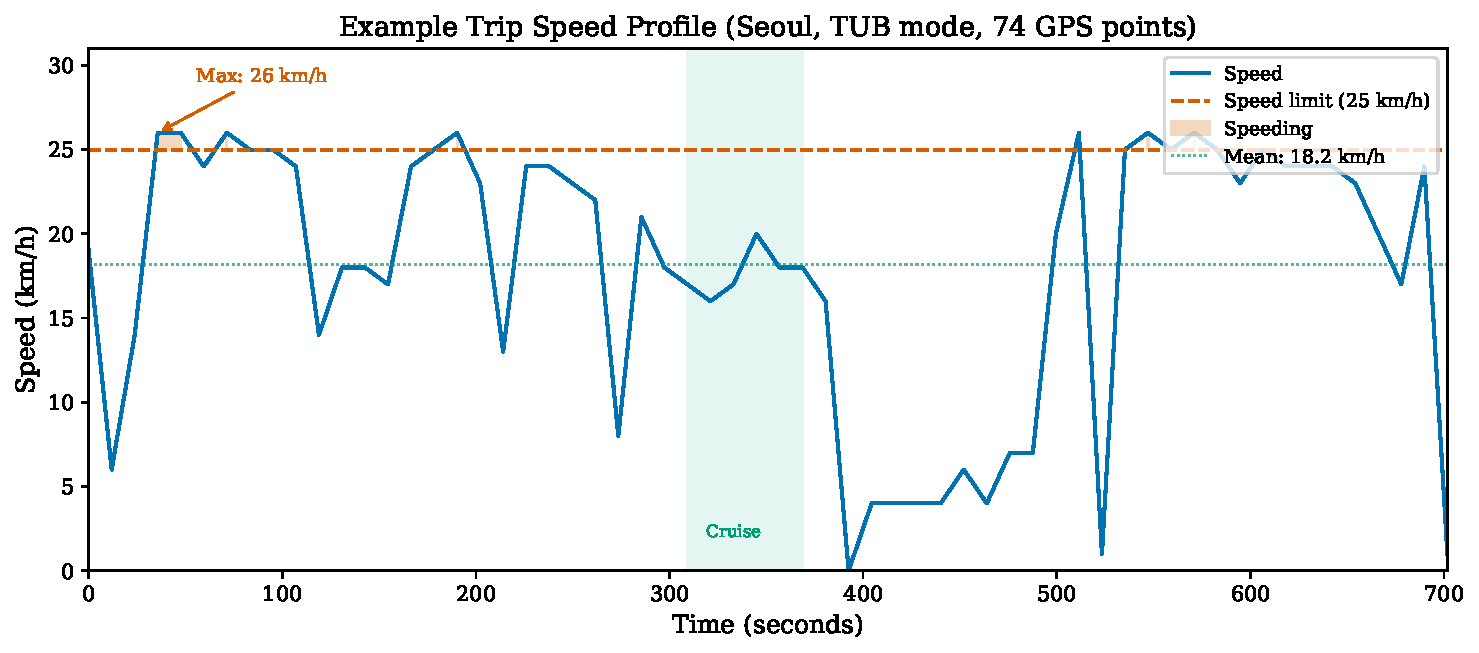
\includegraphics[width=\textwidth]{fig3_speed_profile_example.pdf}
\end{column}
\end{columns}
\end{frame}

% ============================================================
% 4. PHASE 3: MAP-MATCHING & ROAD CLASS
% ============================================================
\section{Phase 3: Road Network Assignment}

\begin{frame}{Phase 3: Map-Matching \& Road Class Assignment}
\textbf{Why}: Link GPS to road infrastructure to study road-type effects on speeding.

\begin{columns}[T]
\begin{column}{0.48\textwidth}
\textbf{Approach evolution}
\begin{enumerate}
\item OSM networks: 50 cities, 1.32M nodes
\item LeuvenMapMatching: 5.8s/trip (infeasible)
\item mappymatch: API incompatible
\item \textbf{DuckDB + KDTree}: 105M pts in 463s
\end{enumerate}
\vspace{0.1cm}
\textbf{Distribution}: residential 41\%, tertiary 15\%, service 15\%, footway 14.5\%, major 13.6\%
\end{column}
\begin{column}{0.50\textwidth}
\centering
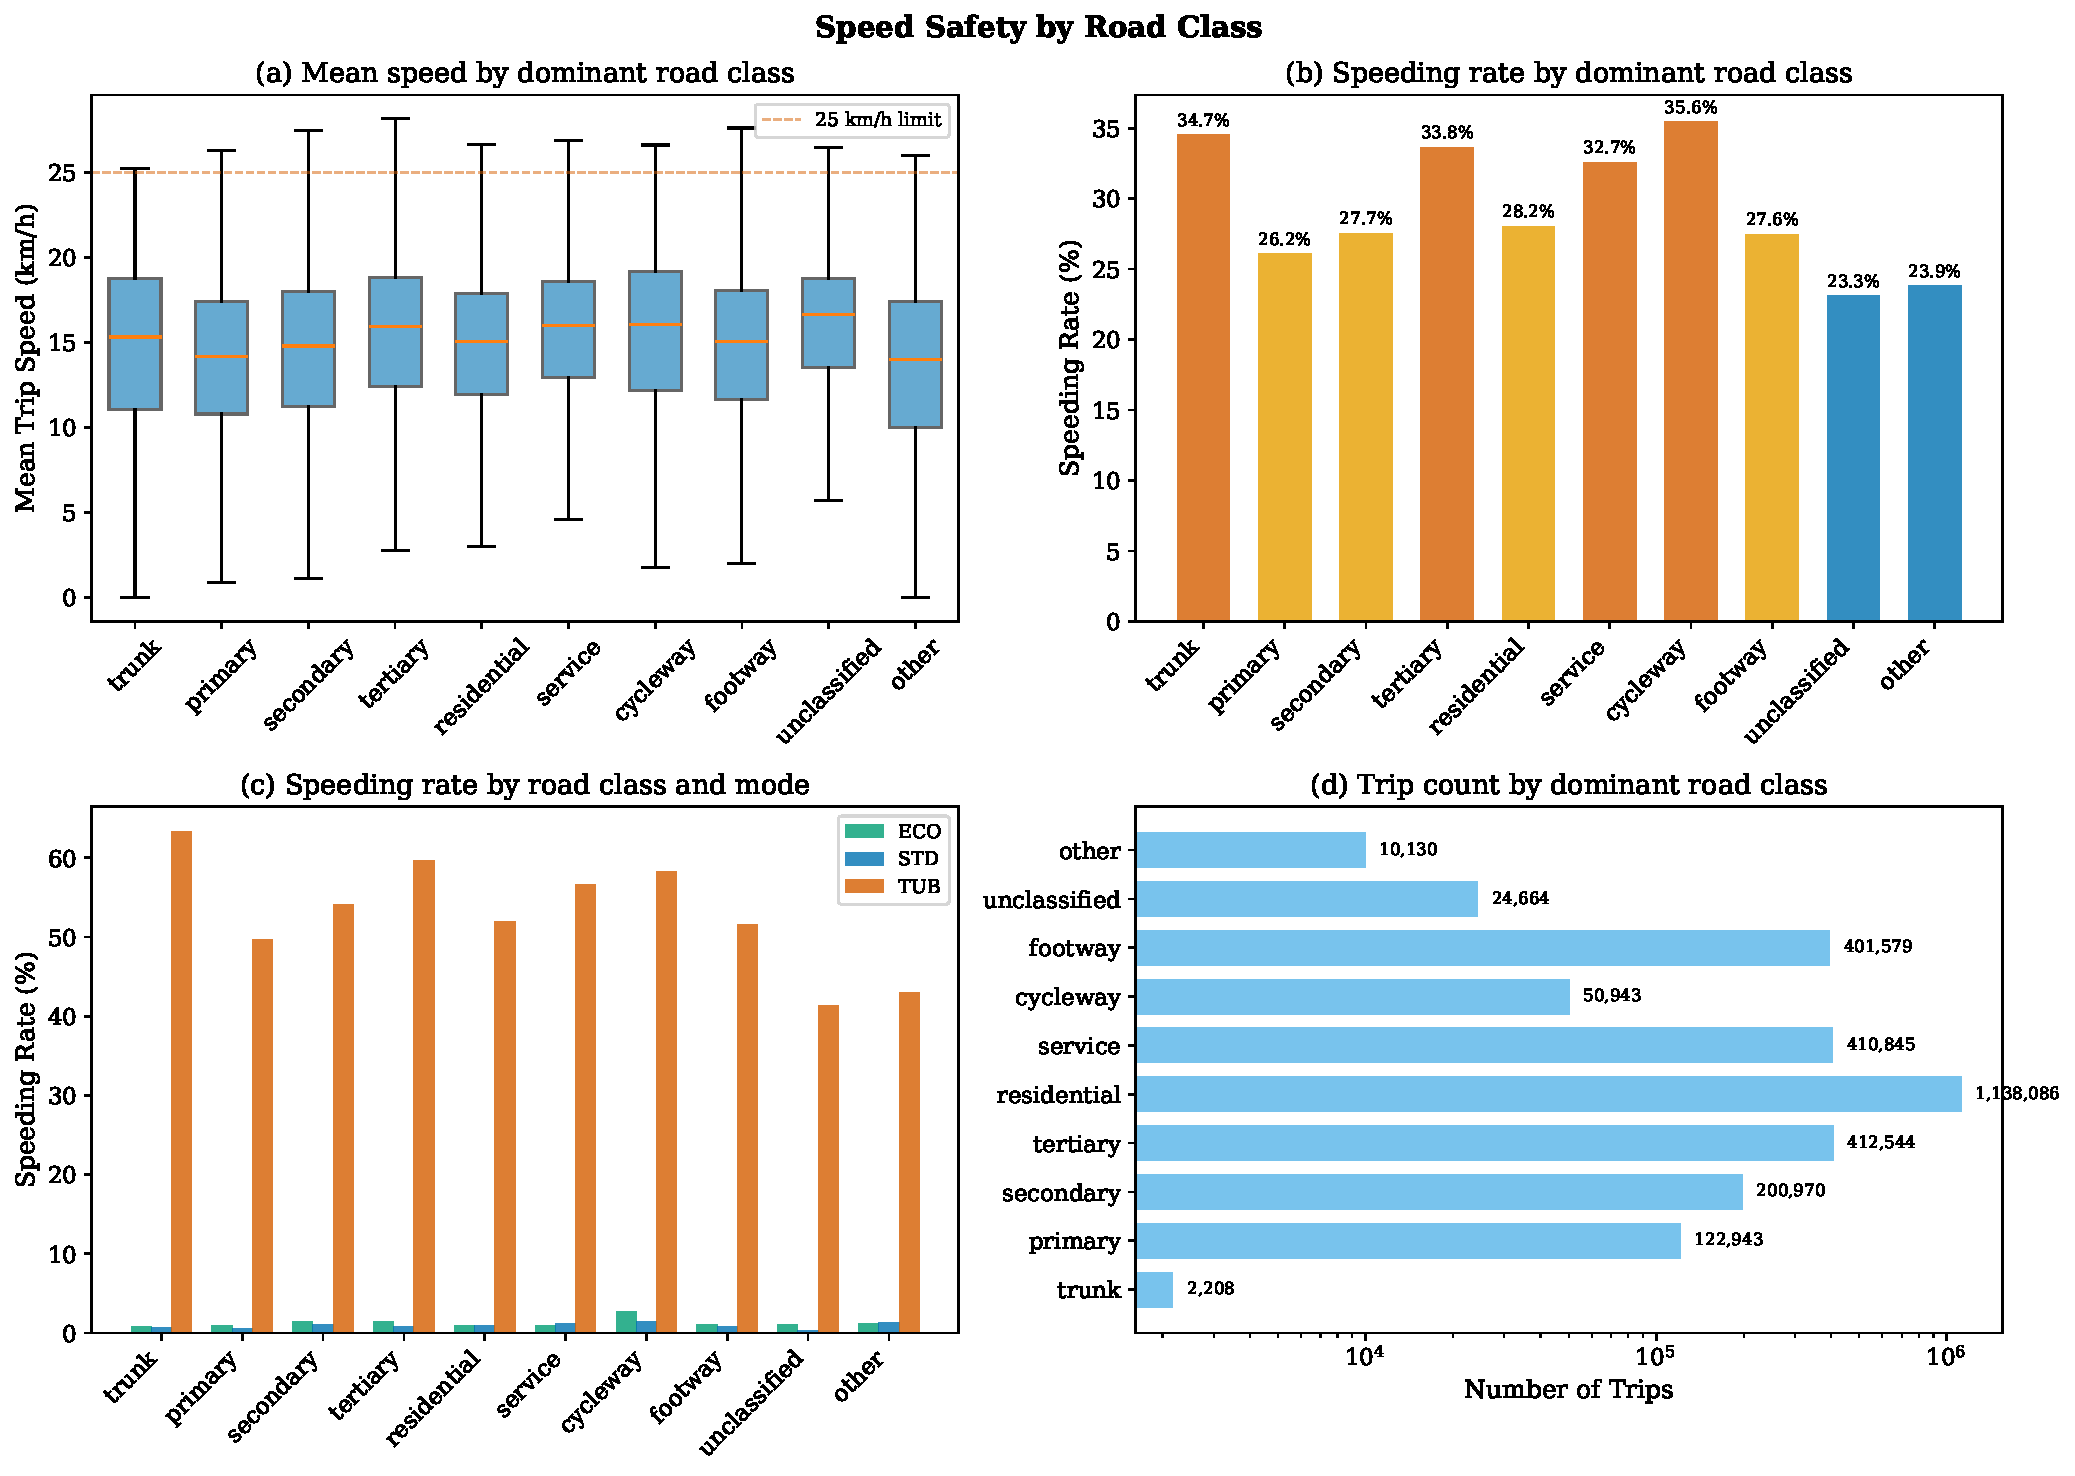
\includegraphics[width=\textwidth]{fig8_speed_by_road_class.pdf}
\end{column}
\end{columns}
\end{frame}

% ============================================================
% 5. PHASE 4: SPATIAL ANALYSIS
% ============================================================
\section{Phase 4: Spatial Analysis}

\begin{frame}{Phase 4: Where Does Speeding Cluster?}
\textbf{Why}: Identify hot spots for targeted enforcement and infrastructure.

\begin{columns}[T]
\begin{column}{0.45\textwidth}
\textbf{Methods}
\begin{itemize}
\item H3 hex grid (res.\ 8, $\sim$461m): 6,111 hexes
\item Getis-Ord Gi* ($k=8$, 999 perms)
\item Global Moran's I + LISA clusters
\end{itemize}
\vspace{0.1cm}
\textbf{Key findings}
\begin{itemize}
\item Seoul: 101 hot / 123 cold spots
\item Hot spots: lower cycling infra
\item Daegu: I = 0.712 (highest)
\end{itemize}
\end{column}
\begin{column}{0.53\textwidth}
\centering
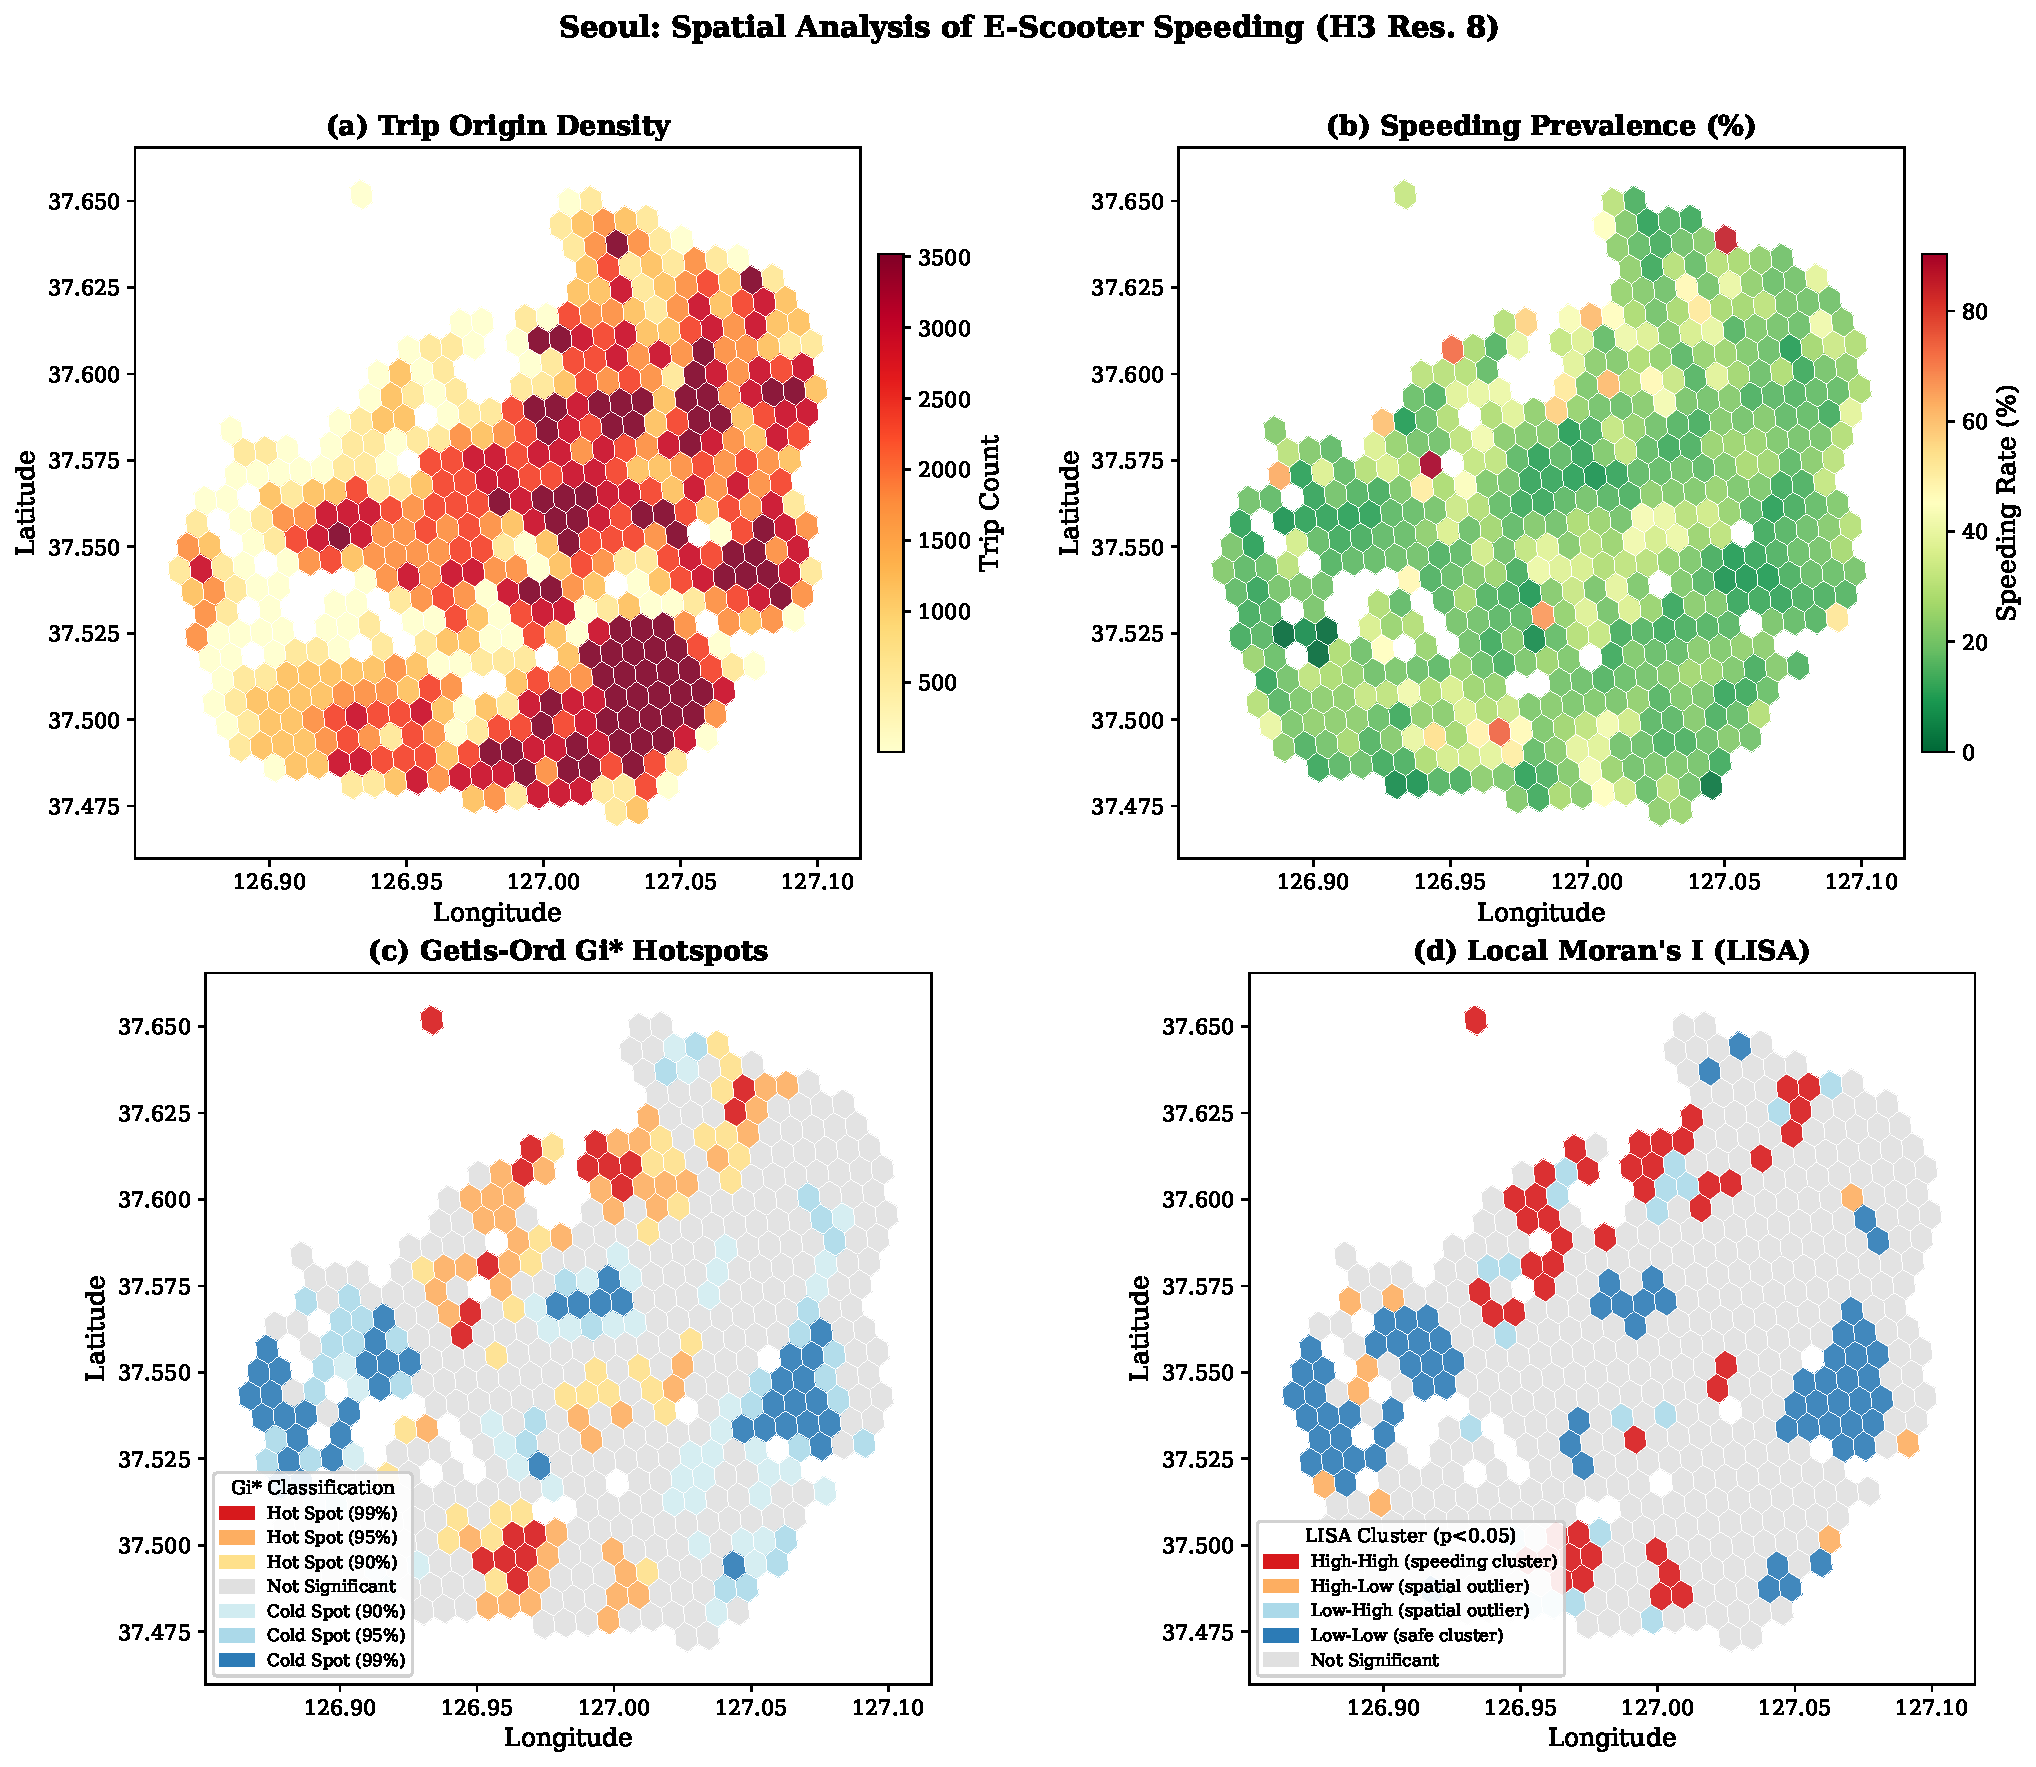
\includegraphics[width=\textwidth]{fig6_seoul_hotspot.pdf}
\end{column}
\end{columns}
\end{frame}

% ============================================================
% 6. PHASE 5: STATISTICAL MODELING
% ============================================================
\section{Phase 5: Statistical Modeling}

\begin{frame}{Phase 5: Model Suite Overview}
\textbf{Why}: Quantify speeding drivers, accounting for user heterogeneity and zero-inflation.

\vspace{0.1cm}
\centering
\footnotesize
\begin{tabular}{@{}clll@{}}
\toprule
\textbf{\#} & \textbf{Model} & \textbf{Purpose} & \textbf{Key Finding} \\
\midrule
1 & Logistic + GEE & Speeding probability & TUB OR = 121 \\
2 & Mixed-effects LM & Mean speed drivers & ICC = 0.271 \\
3 & Two-part hurdle & Zero-inflated speeding & 70.4\% zeros \\
4 & GMM ($K\!=\!4$) & Rider typology & 4 clusters \\
5 & Multinomial logit & Class membership & TUB RRR = 11.8 \\
6 & GEE experience & Learning effect & OR = 1.18/log-trip \\
7 & Spline logistic & Distance--speeding & pseudo-$R^2$=0.39 \\
8 & SHAP/LightGBM & Feature importance & AUC = 0.905 \\
\bottomrule
\end{tabular}
\vspace{0.2cm}

\normalsize \textbf{All models}: TUB mode is the dominant predictor of speeding.
\end{frame}

\begin{frame}{Core Finding: TUB Mode Dominates}
\begin{columns}[T]
\begin{column}{0.48\textwidth}
\centering
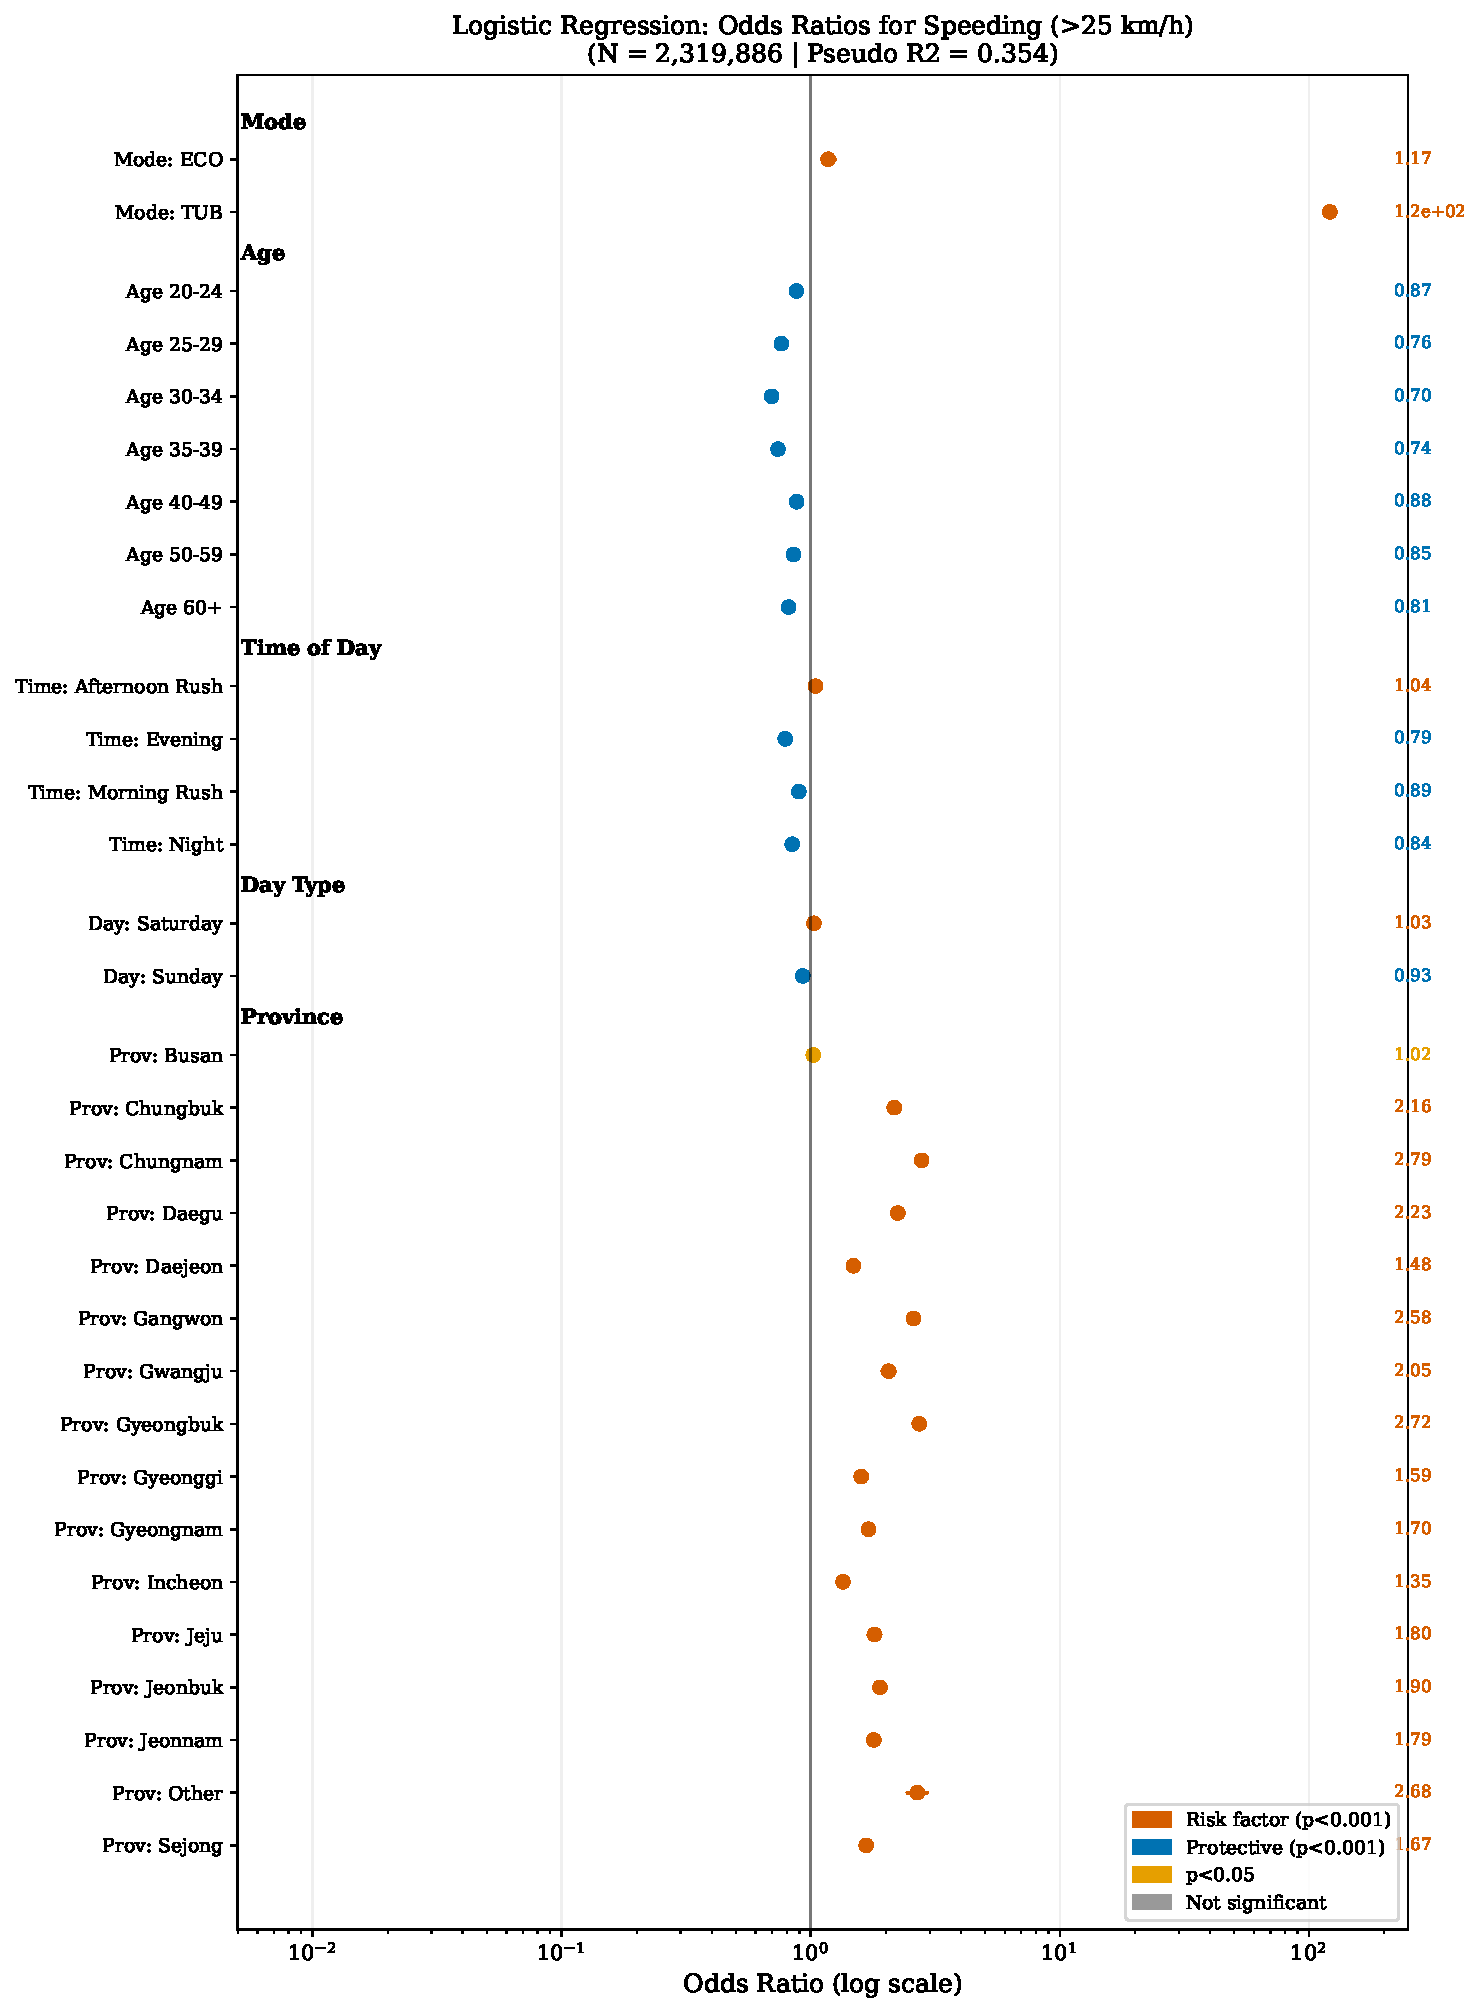
\includegraphics[width=\textwidth,height=0.55\textheight,keepaspectratio]{fig9_logistic_OR.pdf}
\end{column}
\begin{column}{0.48\textwidth}
\centering
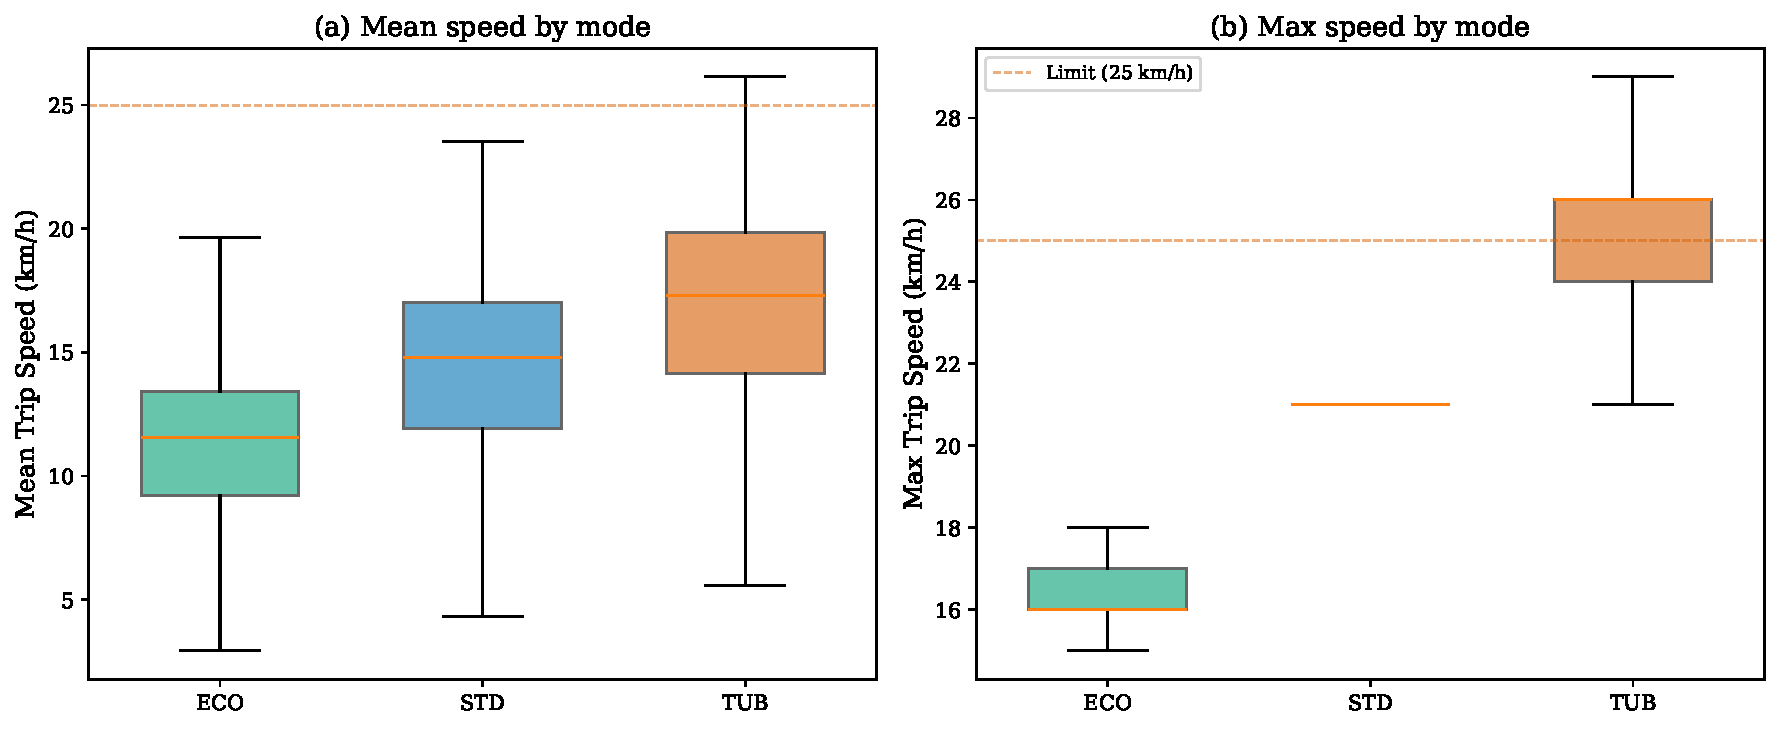
\includegraphics[width=\textwidth,height=0.55\textheight,keepaspectratio]{fig4_speed_by_mode.pdf}
\end{column}
\end{columns}
\vspace{0.1cm}
\begin{itemize}
\item TUB mode OR = 121 for speeding; ECO $\to$ 34\% speed reduction, speeding 54\% $\to$ 1.1\%
\item Within-subject paired ($n=12{,}046$): all effects $p<0.001$
\end{itemize}
\end{frame}

\begin{frame}{Rider Typology: Four Behavioral Clusters}
\begin{columns}[T]
\begin{column}{0.48\textwidth}
\centering
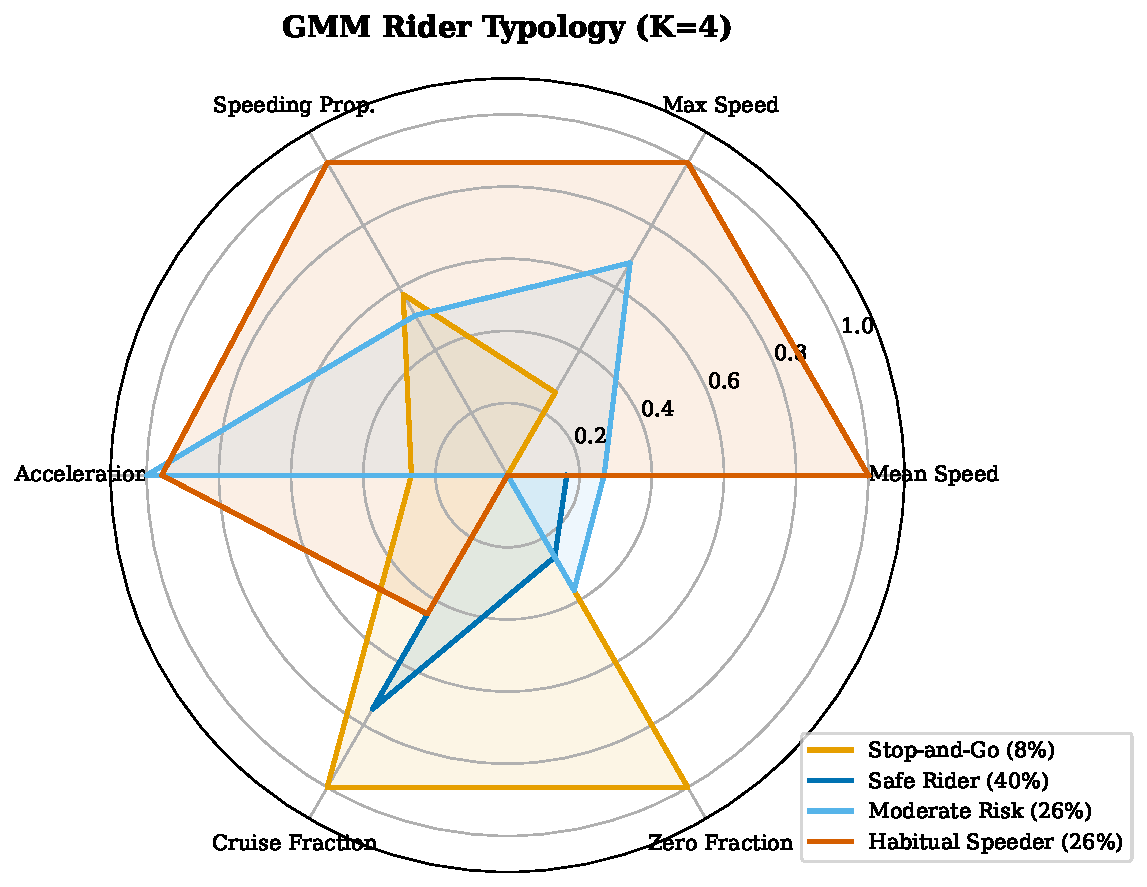
\includegraphics[width=0.95\textwidth]{fig11_rider_typology_radar.pdf}
\end{column}
\begin{column}{0.50\textwidth}
\textbf{GMM $K=4$}: Safe (40\%), Moderate (26\%), Habitual Speeder (26\%), Stop-and-Go (8\%)

\vspace{0.15cm}
\textbf{Multinomial logit} (class membership):
\begin{itemize}
\item TUB: RRR = 11.8 for Speeder class
\item ECO: RRR = 0.06 (protective)
\item Pseudo $R^2$ = 0.297
\end{itemize}
\end{column}
\end{columns}
\end{frame}

\begin{frame}{Robustness: Findings Hold Across Tests}
\begin{columns}[T]
\begin{column}{0.32\textwidth}
\centering
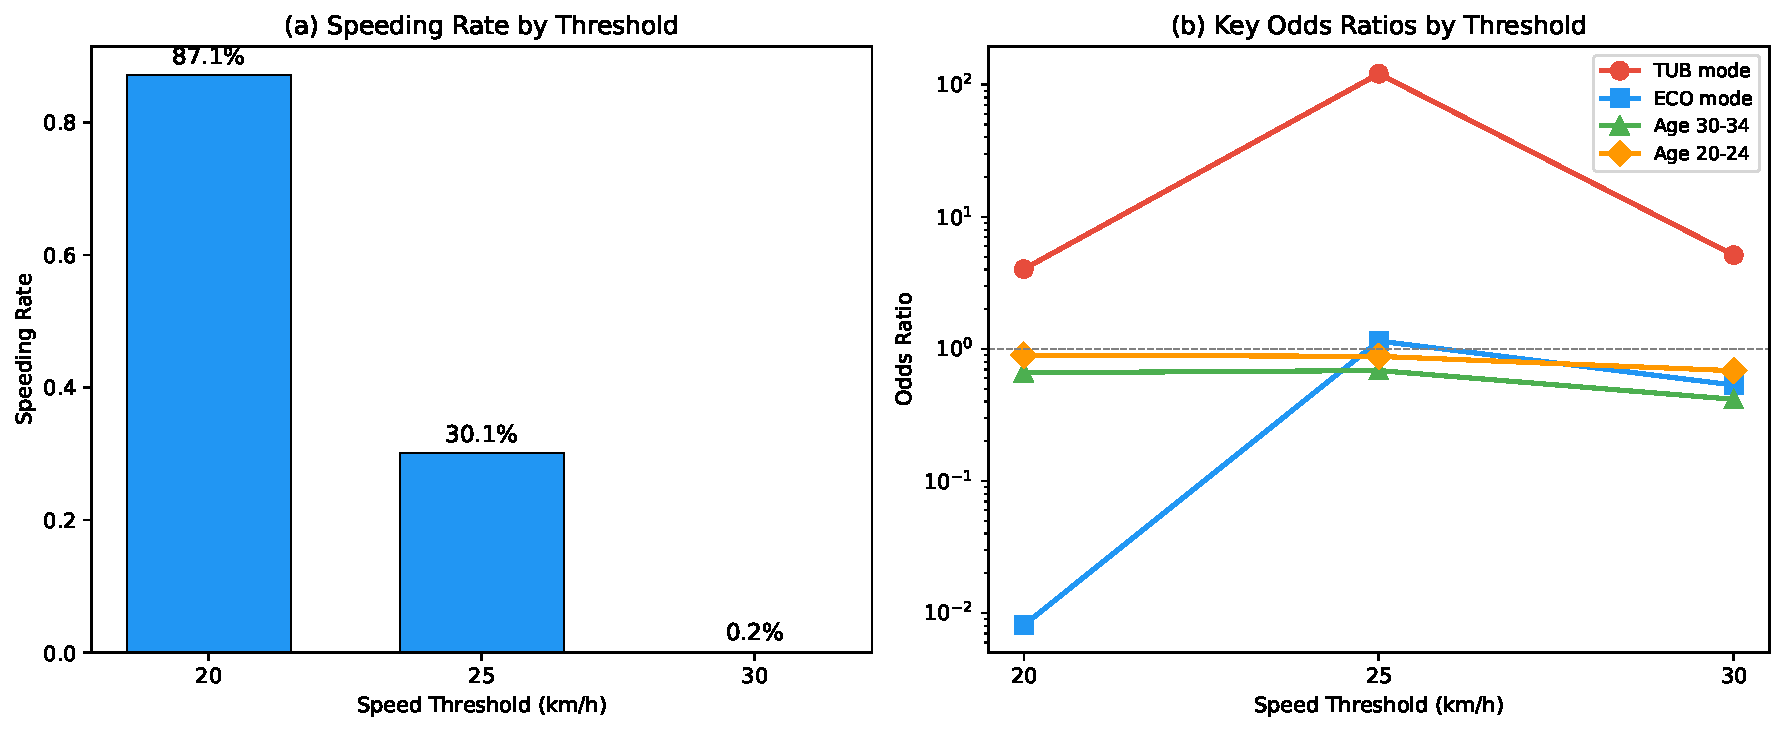
\includegraphics[width=\textwidth]{robustness_threshold.pdf}
\vspace{0.1cm}
\footnotesize \textbf{Threshold sensitivity}\\20 km/h: 87\%\\25 km/h: 30\%\\30 km/h: 0.2\%
\end{column}
\begin{column}{0.32\textwidth}
\centering
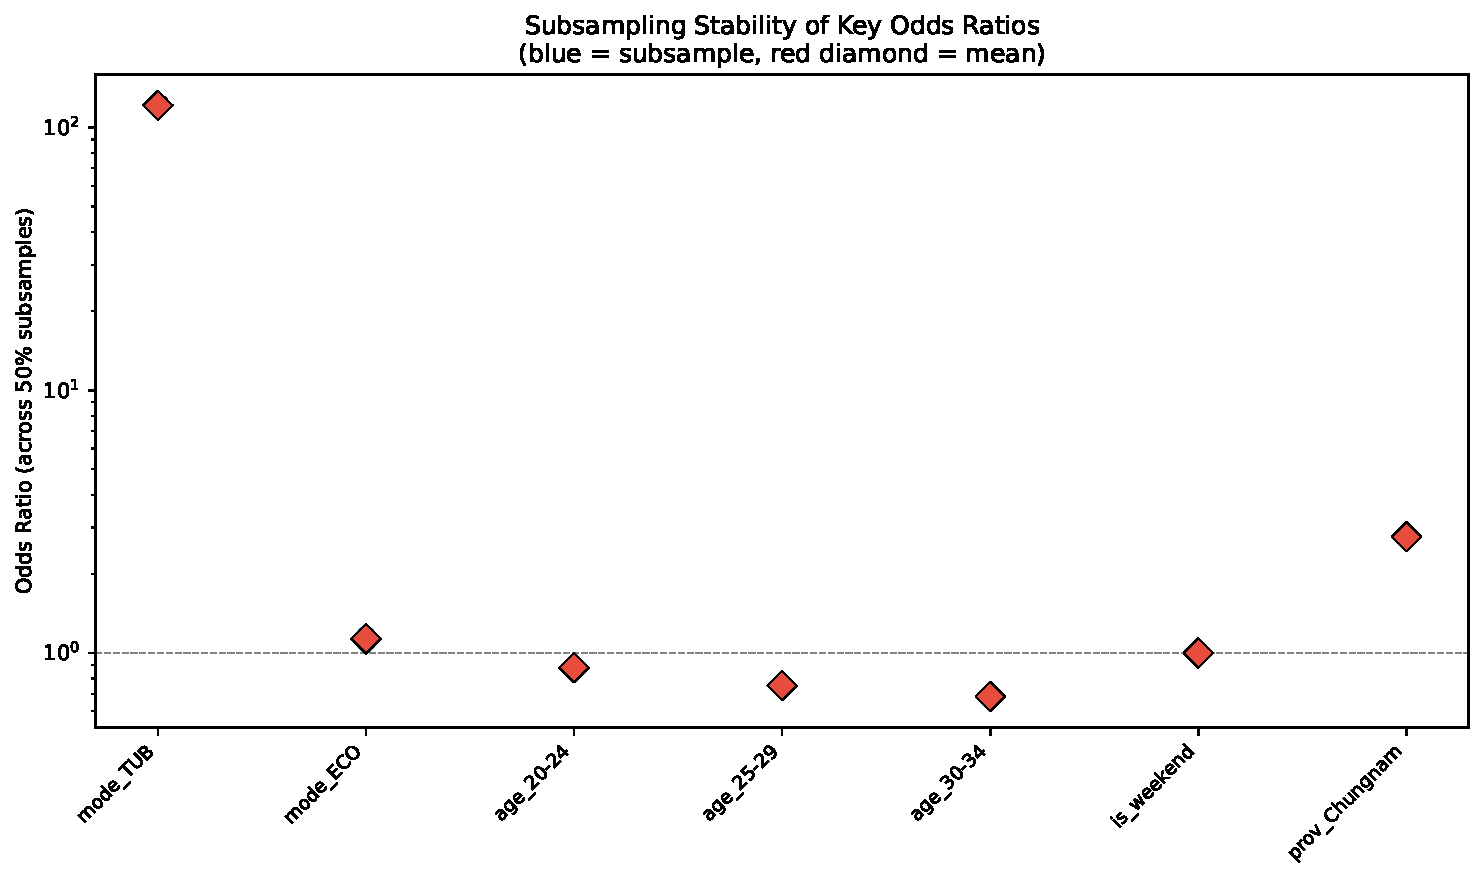
\includegraphics[width=\textwidth]{robustness_subsampling.pdf}
\vspace{0.1cm}
\footnotesize \textbf{Subsampling stability}\\TUB OR CV $<$ 1.2\%\\across 5 folds
\end{column}
\begin{column}{0.32\textwidth}
\centering
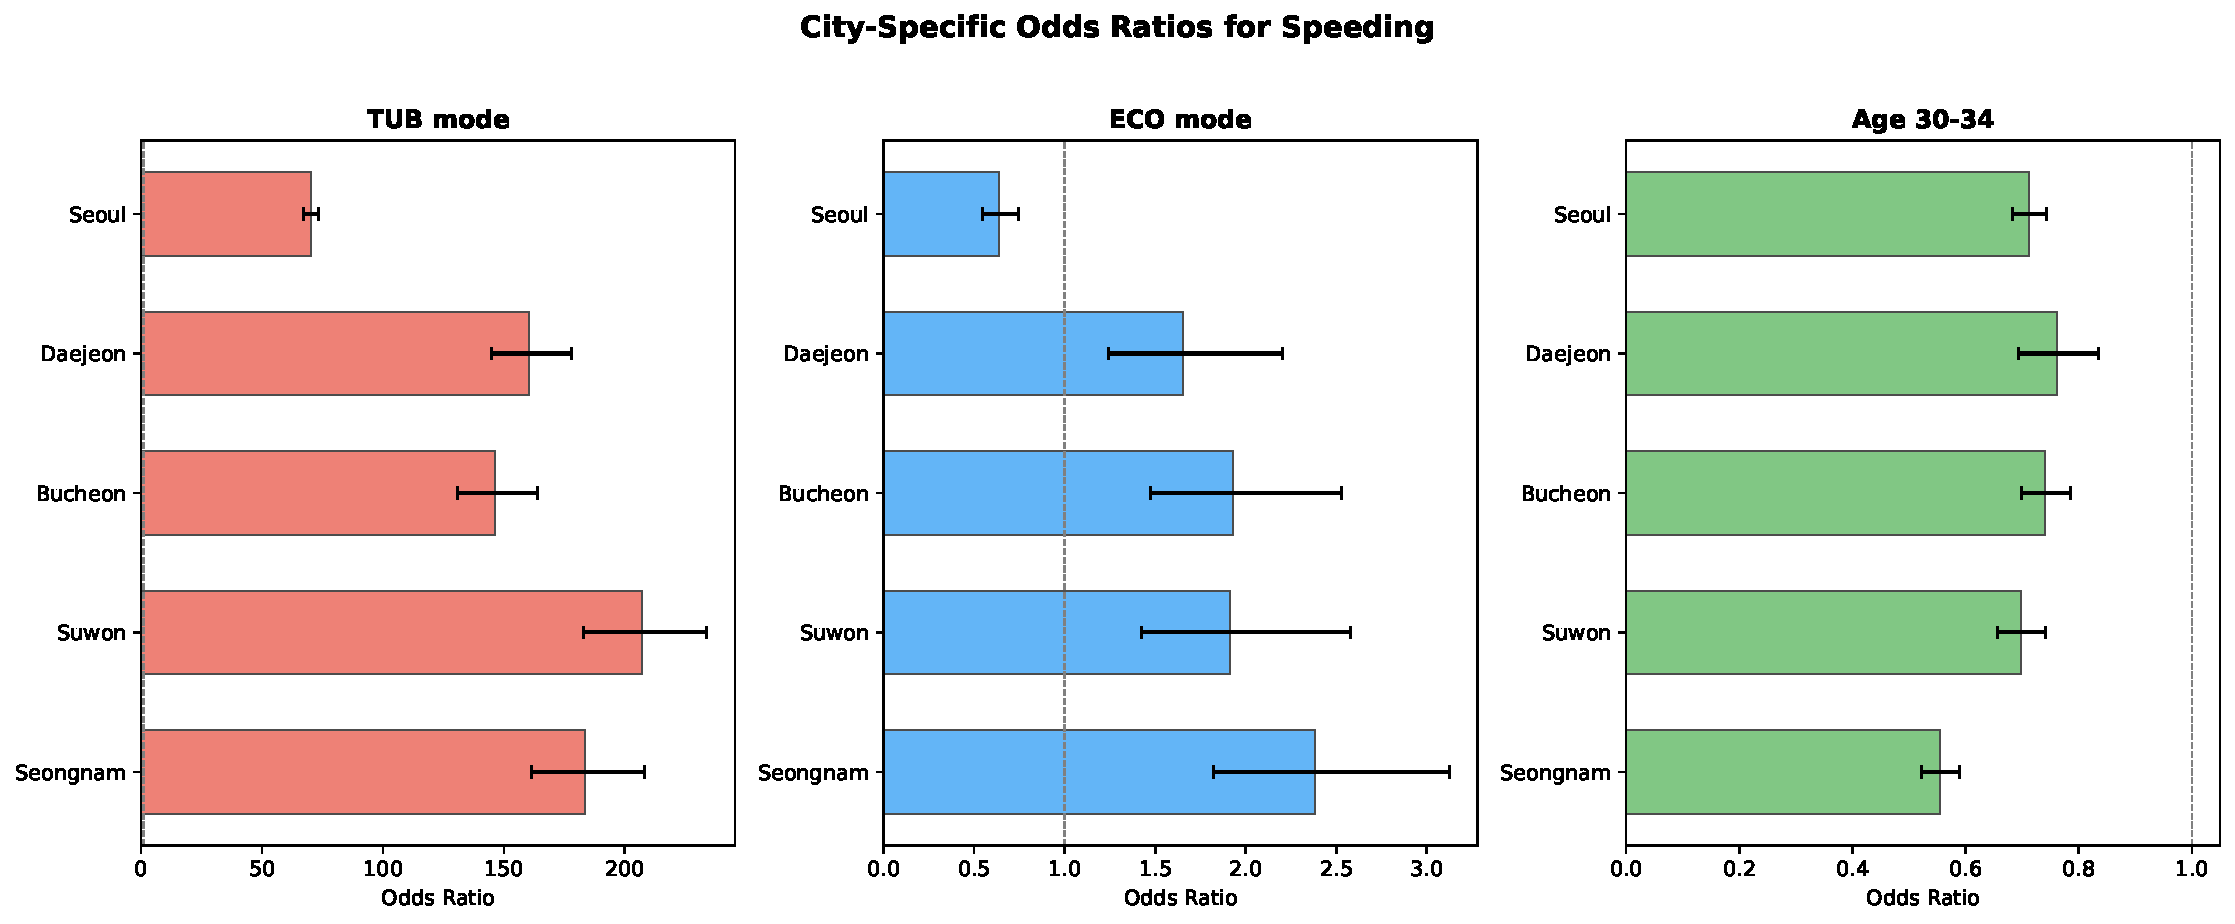
\includegraphics[width=\textwidth]{robustness_city_models.pdf}
\vspace{0.1cm}
\footnotesize \textbf{City-specific models}\\TUB OR range: 70--207\\across 5 cities
\end{column}
\end{columns}
\end{frame}

% ============================================================
% 7. PHASE 8: EXTENSION ANALYSES
% ============================================================
\section{Phase 8: Extension Analyses}

\begin{frame}{Phase 8: Five Extension Research Questions}
\textbf{Why}: Extend to 24-month longitudinal data (44.1M trips) for deeper insights.

\begin{columns}[T]
\begin{column}{0.48\textwidth}
\textbf{8.1 Experience effect}
\begin{itemize}
\item Speeding: 3.8\% (trip 1) $\to$ 28\% (500+)
\item \alert{But}: via TUB adoption, not skill
\item TUB use: 11.5\% $\to$ 47.8\% over 50 trips
\end{itemize}
\vspace{0.1cm}
\textbf{8.2 Trip distance}
\begin{itemize}
\item 13.9\% (149m) $\to$ 54.2\% (2168m)
\item Speed drift: $-1.5$ km/h in 2nd half
\end{itemize}
\end{column}
\begin{column}{0.48\textwidth}
\textbf{8.3 Road curvature}
\begin{itemize}
\item More curves $\to$ less speeding (OR=0.716)
\item Risk 5$\times$ higher when speeding on curves
\end{itemize}
\vspace{0.1cm}
\textbf{8.4 SHAP interpretability}
\begin{itemize}
\item LightGBM AUC = 0.905
\item TUB SHAP = 2.33 (3.6$\times$ next)
\end{itemize}
\end{column}
\end{columns}
\end{frame}

\begin{frame}{Experience Effect: It's About Mode Adoption}
\begin{columns}[T]
\begin{column}{0.48\textwidth}
\centering
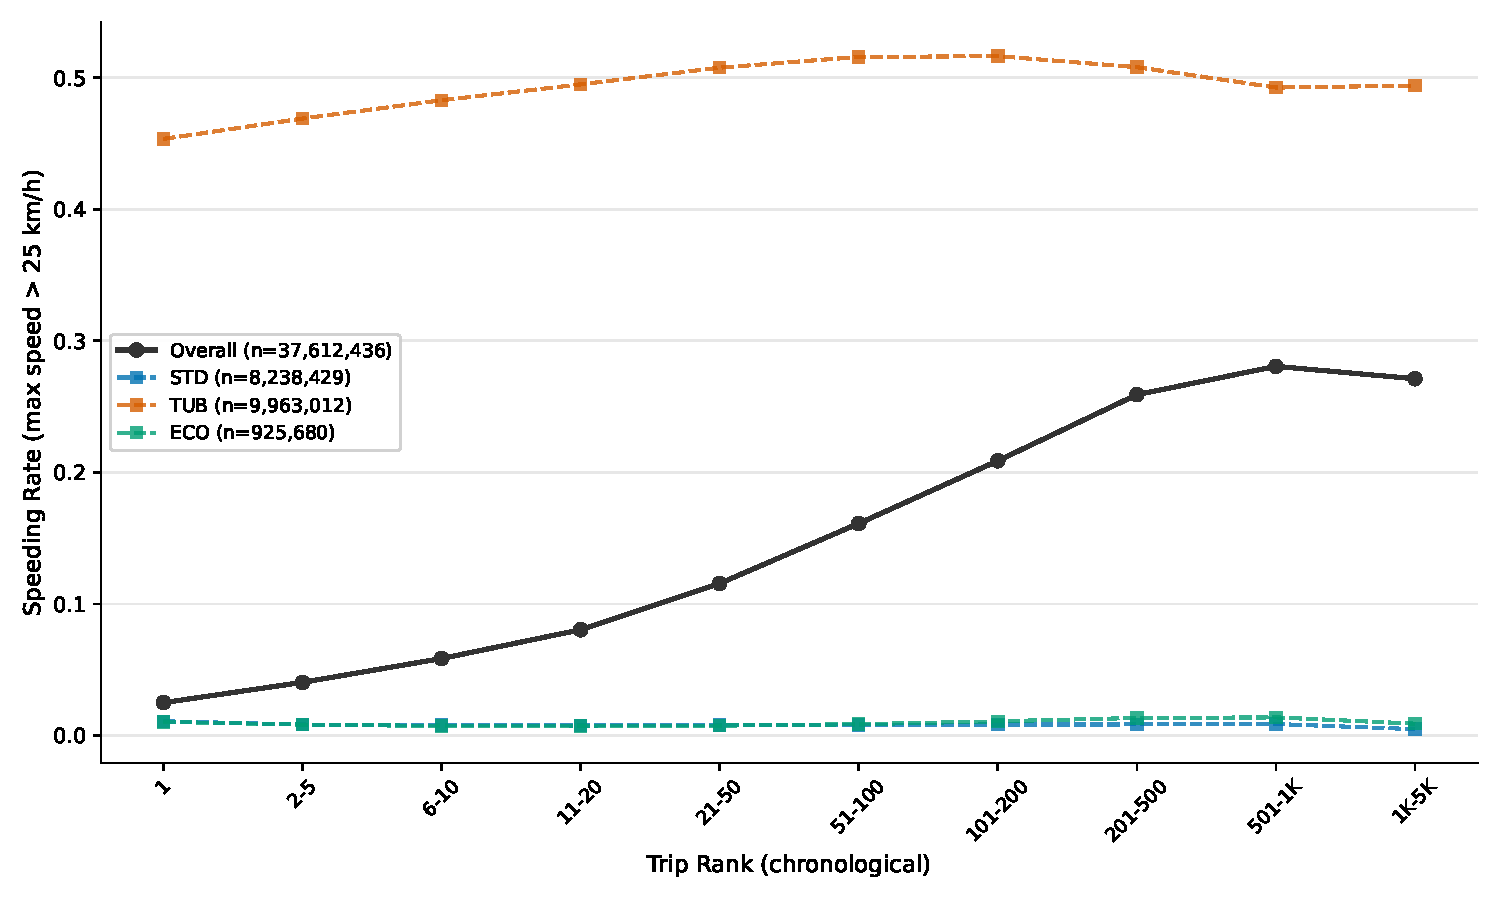
\includegraphics[width=\textwidth]{fig_experience_learning_curve.pdf}
\vspace{0.1cm}
\footnotesize Speeding rate by experience level
\end{column}
\begin{column}{0.48\textwidth}
\centering
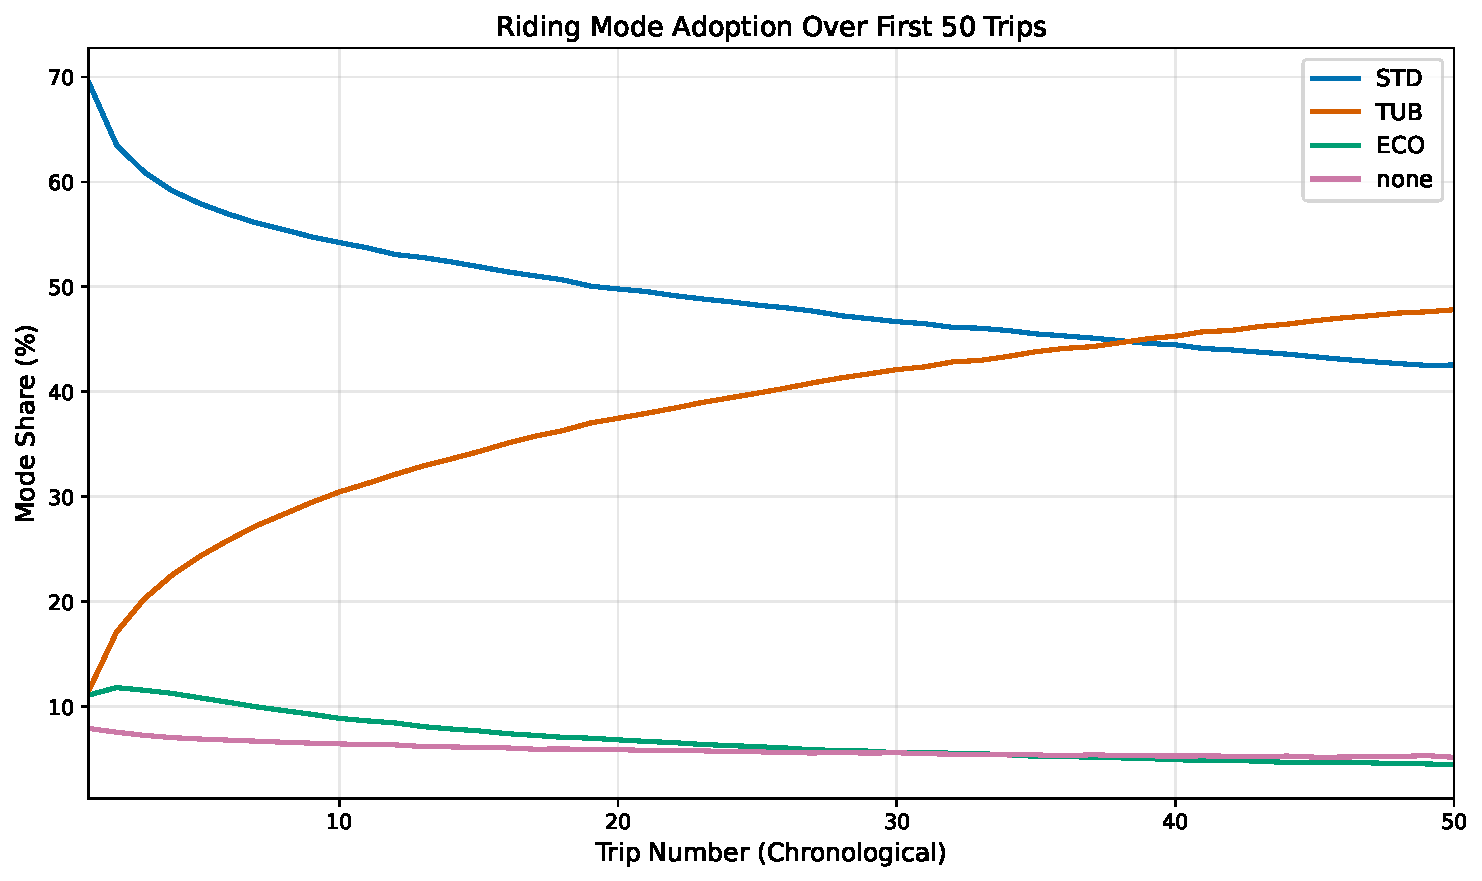
\includegraphics[width=\textwidth]{fig_newcomer_mode_adoption.pdf}
\vspace{0.1cm}
\footnotesize TUB adoption over first 50 trips
\end{column}
\end{columns}
\vspace{0.3cm}
\centering
Within STD/ECO modes only: speeding is virtually constant across experience (0.8--1.5\%).\\
$\Rightarrow$ \textbf{98.4\% of the experience--speeding gradient is mediated by TUB adoption.}
\end{frame}

\begin{frame}{SHAP: TUB Mode Dwarfs All Other Features}
\begin{columns}[T]
\begin{column}{0.48\textwidth}
\centering
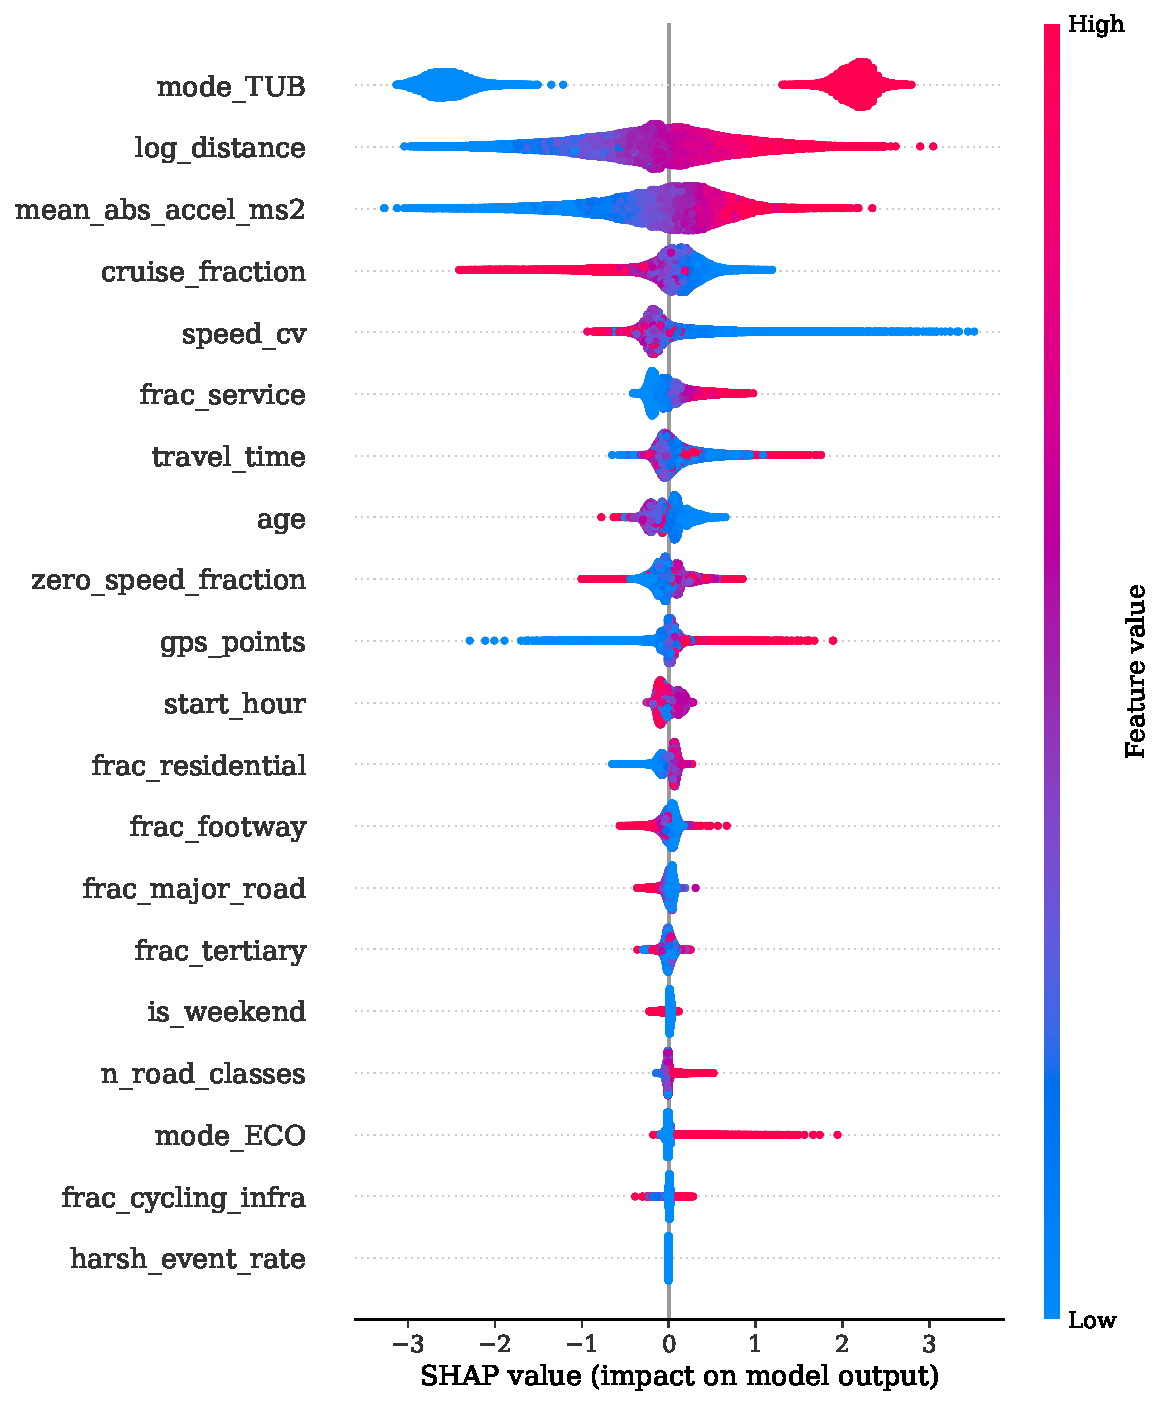
\includegraphics[width=\textwidth,height=0.7\textheight,keepaspectratio]{fig_shap_summary.pdf}
\end{column}
\begin{column}{0.48\textwidth}
\centering
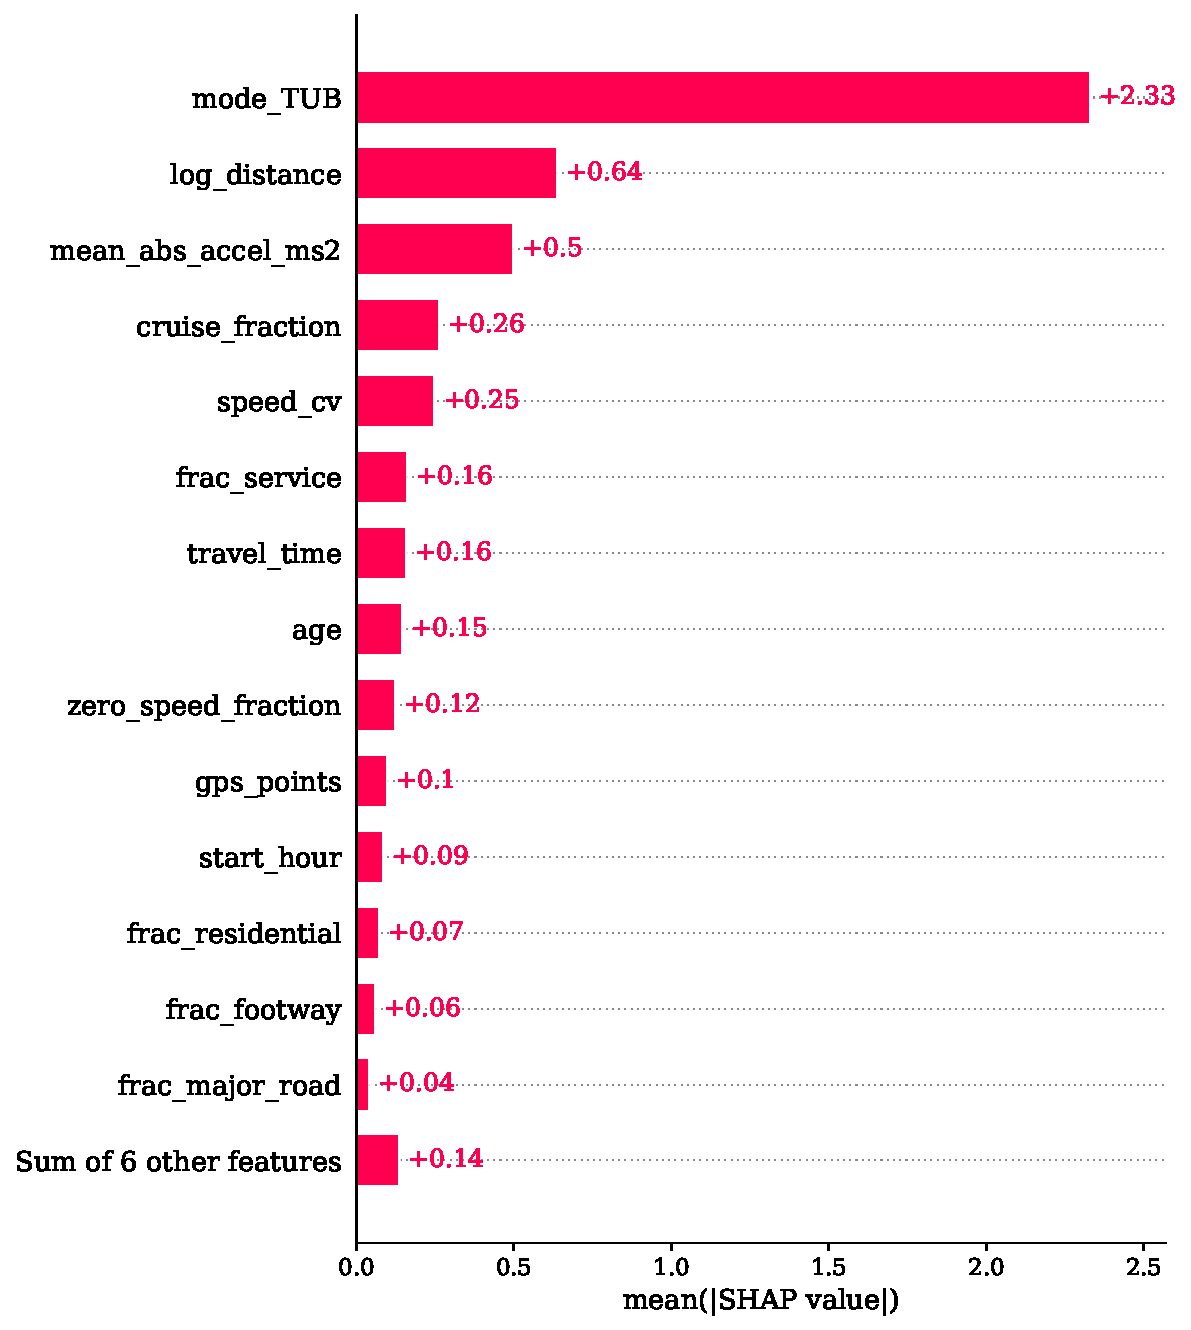
\includegraphics[width=\textwidth,height=0.7\textheight,keepaspectratio]{fig_shap_bar.pdf}
\end{column}
\end{columns}
\centering
\footnotesize TUB mean $|\text{SHAP}|$ = 2.33 vs.\ 0.64 (log distance) --- 3.6$\times$ gap.
\end{frame}

% ============================================================
% 8. PHASE 11: DiD CAUSAL ANALYSIS
% ============================================================
\section{Phase 11: DiD Causal Analysis}

\begin{frame}{Phase 11: The December 2023 Natural Experiment}
\textbf{Why}: From association to \textbf{causation}. Dec 2023 TUB ban = clean quasi-experiment.

\begin{columns}[T]
\begin{column}{0.48\textwidth}
\centering
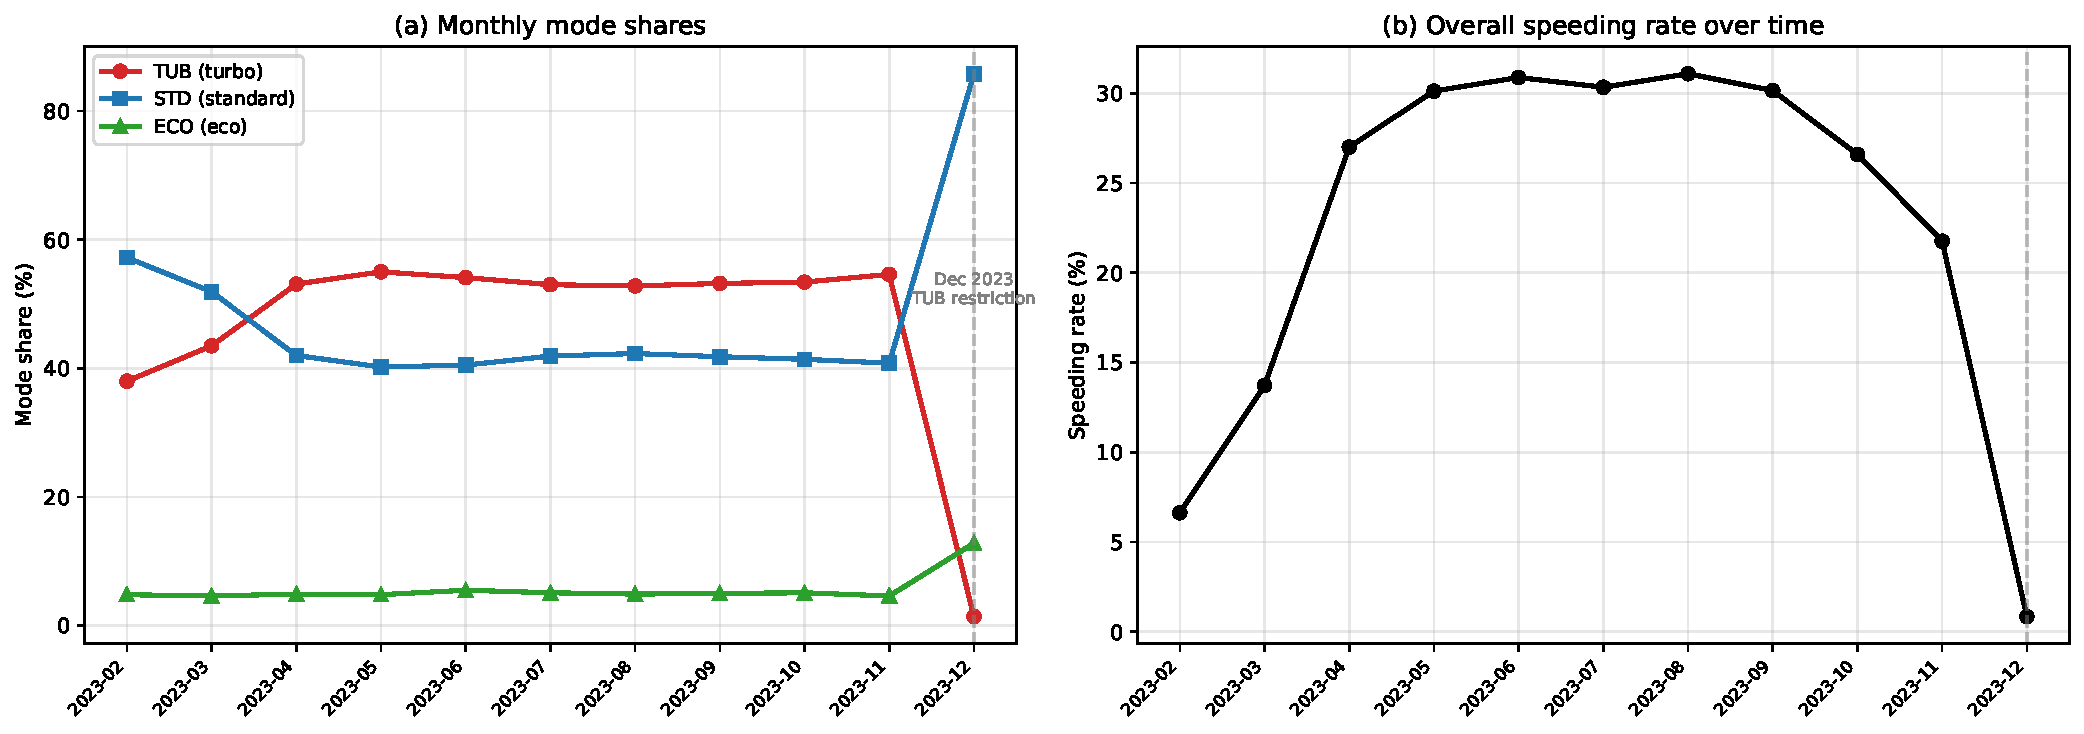
\includegraphics[width=\textwidth,height=0.65\textheight,keepaspectratio]{fig_did_mode_trends.pdf}
\end{column}
\begin{column}{0.50\textwidth}
\textbf{Treatment}: System-wide TUB ban
\begin{itemize}
\item TUB: 54.6\% $\to$ 1.4\%
\item STD absorbed: 40.8\% $\to$ 85.8\%
\item 50/54 cities $>$10pp TUB drop
\end{itemize}
\vspace{0.1cm}
\textbf{ID}: Cross-city TUB share variation\\
\textbf{Panel}: 53 cities $\times$ 11 months
\end{column}
\end{columns}
\end{frame}

\begin{frame}{DiD Results: Causal Speed Reduction}
\begin{columns}[T]
\begin{column}{0.48\textwidth}
\centering
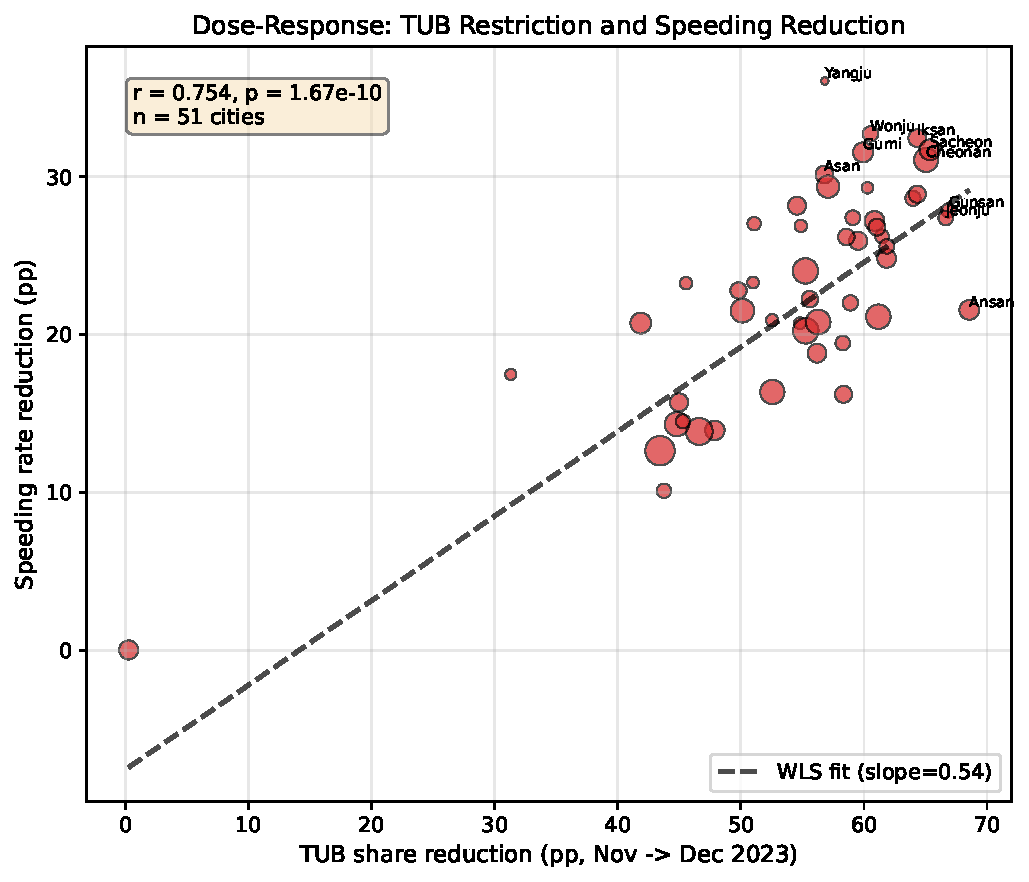
\includegraphics[width=\textwidth,height=0.55\textheight,keepaspectratio]{fig_did_dose_response.pdf}
\end{column}
\begin{column}{0.48\textwidth}
\centering
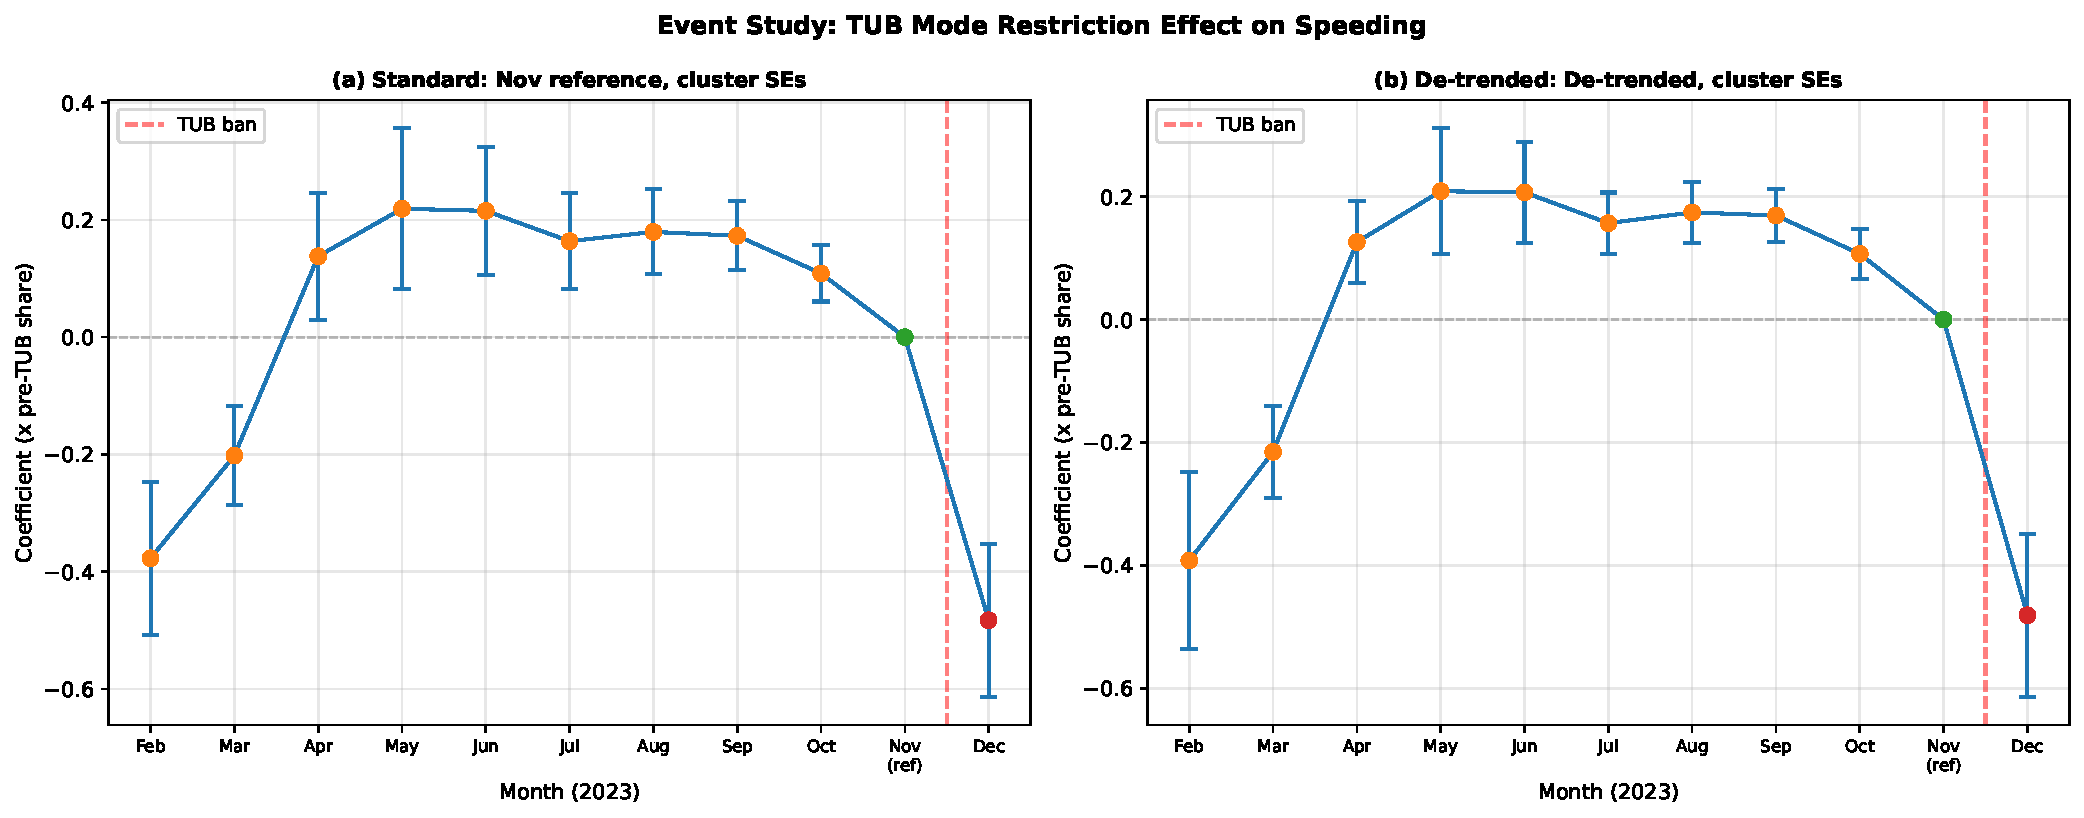
\includegraphics[width=\textwidth,height=0.55\textheight,keepaspectratio]{fig_did_event_study_v2.pdf}
\end{column}
\end{columns}
\vspace{0.1cm}
\begin{itemize}
\item \textbf{TWFE}: $\beta\!=\!-0.568$ --- 50\% pre-TUB city $\to$ 28.4pp reduction
\item \textbf{Dose-response}: 10pp TUB $\to$ 5.0pp speeding ($r\!=\!0.754$)
\item \textbf{Placebo}: $\beta\!=\!-0.015$, $p\!=\!0.561$ --- \textbf{PASS}
\end{itemize}
\end{frame}

\begin{frame}{Behavioral Substitution: No Risk Compensation}
\textbf{Why}: Does banning TUB make riders speed more in STD? (Risk compensation)

\begin{columns}[T]
\begin{column}{0.45\textwidth}
\centering
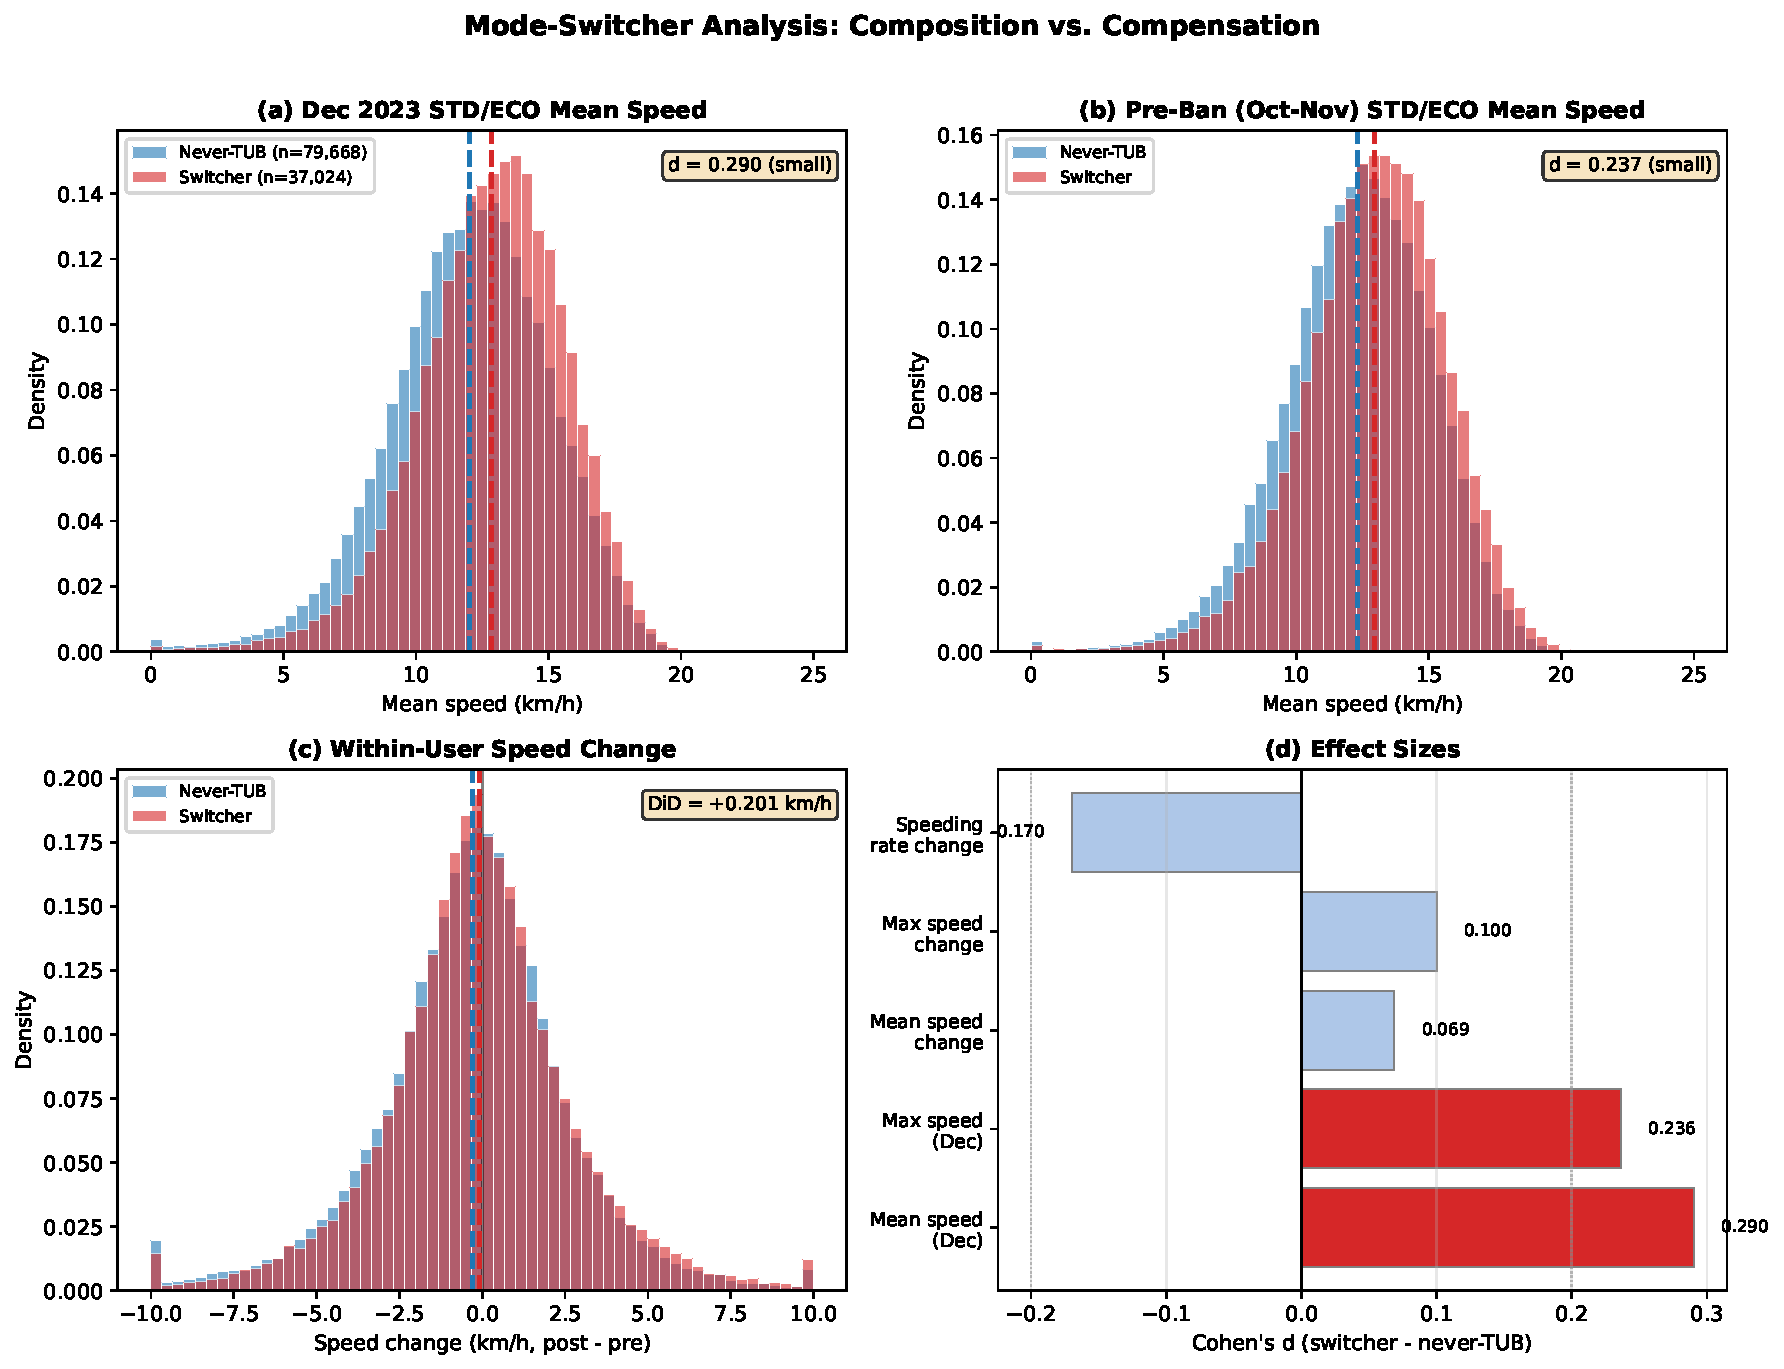
\includegraphics[width=\textwidth]{fig_mode_switcher.pdf}
\end{column}
\begin{column}{0.52\textwidth}
\textbf{Multi-outcome DiD}
\begin{itemize}
\item Overall speeding: $\beta\!=\!-0.568$ \checkmark
\item Trip distance: n.s.\ ($p\!=\!0.45$)
\item STD/ECO speeding: n.s.\ ($p\!=\!0.59$)
\item STD/ECO speed: $+0.85$ km/h (composition)
\end{itemize}
\vspace{0.1cm}
\textbf{Mode-switcher} ($n = 120$K)
\begin{itemize}
\item Within-user: $+0.20$ km/h ($d\!=\!0.069$)
\item \textbf{Verdict}: Composition, not compensation
\end{itemize}
\end{column}
\end{columns}
\end{frame}

% ============================================================
% 9. PHASE 12: SURVIVAL ANALYSIS
% ============================================================
\section{Phase 12: Survival Analysis}

\begin{frame}{Phase 12: Time-to-First-Speeding}
\textbf{Why}: When do riders first cross 25 km/h? Survival analysis reveals onset dynamics.

\begin{columns}[T]
\begin{column}{0.48\textwidth}
\centering
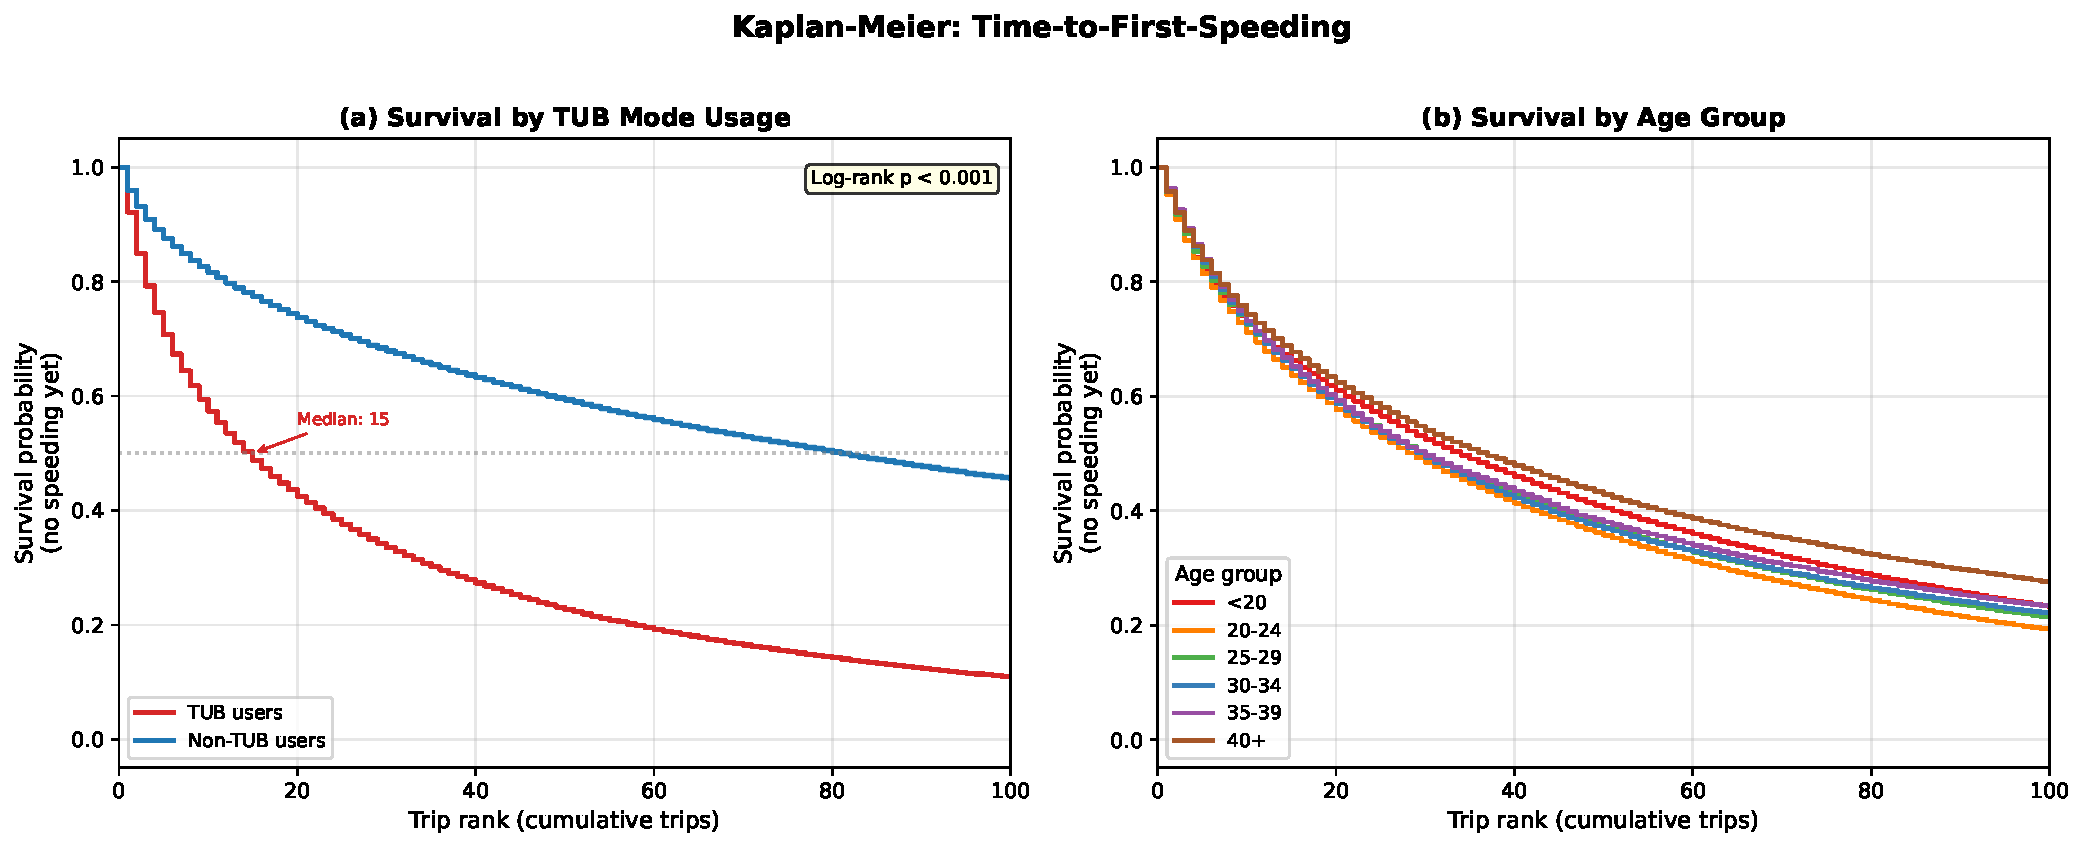
\includegraphics[width=\textwidth]{fig_survival_km.pdf}
\end{column}
\begin{column}{0.50\textwidth}
\textbf{864K users} ($\geq$2 trips): 48\% event, 52\% censored
\vspace{0.1cm}
\begin{itemize}
\item TUB: median \textbf{15 trips} to first speeding
\item Non-TUB: median \textbf{81 trips} (5.4$\times$)
\item Log-rank $\chi^2 = 91{,}282$
\item Cox TV: TUB HR = \textbf{10.41}
\end{itemize}
\vspace{0.1cm}
\textbf{98.4\%} of experience--speeding gradient mediated by TUB adoption
\end{column}
\end{columns}
\end{frame}

% ============================================================
% 10. PAPER STATUS
% ============================================================
\section{Paper Status \& Next Steps}

\begin{frame}{Paper: Submission-Ready Manuscript}
\begin{columns}[T]
\begin{column}{0.48\textwidth}
\textbf{Status}
\begin{itemize}
\item $\sim$8,945 words (TR-C: 8--12K)
\item 79 pages, 0 \LaTeX{} errors
\item 9 models + DiD + survival
\item 49+ figures, 51 bib entries (100\% verified)
\item Overleaf synced via git subtree
\end{itemize}
\vspace{0.1cm}
\textbf{QA}: 49\% of bib entries corrected; 3 unverifiable refs replaced; orphans removed
\end{column}
\begin{column}{0.48\textwidth}
\textbf{All sections complete}
\begin{itemize}
\item[\checkmark] Abstract \& Highlights
\item[\checkmark] Introduction (8 contributions)
\item[\checkmark] Literature Review
\item[\checkmark] Data Description (2 tables)
\item[\checkmark] Methodology (9 models)
\item[\checkmark] Results (8 subsections)
\item[\checkmark] Discussion (5 policy recs)
\item[\checkmark] Conclusions + Appendix
\end{itemize}
\end{column}
\end{columns}
\end{frame}

\begin{frame}{Progress Timeline}
\centering
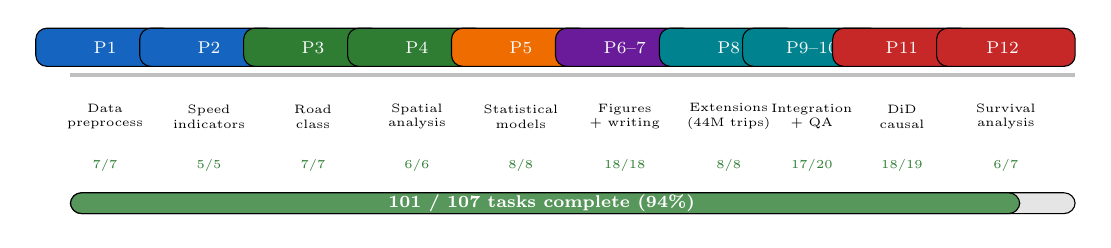
\begin{tikzpicture}[scale=0.88, transform shape,
  phase/.style={draw, rounded corners, minimum width=2cm, minimum height=0.55cm, font=\scriptsize, align=center, text=white},
  label/.style={font=\tiny, align=center, text width=2cm}
]
% Timeline
\draw[very thick, gray!50] (0,0) -- (14.5,0);

% Phase markers
\foreach \x/\c/\t in {
  0.5/PhaseBlue/P1,
  2.0/PhaseBlue/P2,
  3.5/PhaseGreen/P3,
  5.0/PhaseGreen/P4,
  6.5/PhaseOrange/P5,
  8.0/PhasePurple/P6--7,
  9.5/PhaseTeal/P8,
  10.7/PhaseTeal/P9--10,
  12.0/PhaseRed/P11,
  13.5/PhaseRed/P12
} {
  \node[phase, fill=\c] at (\x, 0.4) {\t};
}

% Labels below
\node[label] at (0.5, -0.6) {Data\\preprocess};
\node[label] at (2.0, -0.6) {Speed\\indicators};
\node[label] at (3.5, -0.6) {Road\\class};
\node[label] at (5.0, -0.6) {Spatial\\analysis};
\node[label] at (6.5, -0.6) {Statistical\\models};
\node[label] at (8.0, -0.6) {Figures\\+ writing};
\node[label] at (9.5, -0.6) {Extensions\\(44M trips)};
\node[label] at (10.7, -0.6) {Integration\\+ QA};
\node[label] at (12.0, -0.6) {DiD\\causal};
\node[label] at (13.5, -0.6) {Survival\\analysis};

% Task counts
\node[font=\tiny, AccentGreen] at (0.5, -1.3) {7/7};
\node[font=\tiny, AccentGreen] at (2.0, -1.3) {5/5};
\node[font=\tiny, AccentGreen] at (3.5, -1.3) {7/7};
\node[font=\tiny, AccentGreen] at (5.0, -1.3) {6/6};
\node[font=\tiny, AccentGreen] at (6.5, -1.3) {8/8};
\node[font=\tiny, AccentGreen] at (8.0, -1.3) {18/18};
\node[font=\tiny, AccentGreen] at (9.5, -1.3) {8/8};
\node[font=\tiny, AccentGreen] at (10.7, -1.3) {17/20};
\node[font=\tiny, AccentGreen] at (12.0, -1.3) {18/19};
\node[font=\tiny, AccentGreen] at (13.5, -1.3) {6/7};

% Overall progress bar
\draw[fill=gray!20, rounded corners] (0, -2.0) rectangle (14.5, -1.7);
\draw[fill=AccentGreen!80, rounded corners] (0, -2.0) rectangle (13.7, -1.7);
\node[font=\scriptsize\bfseries, white] at (6.8, -1.85) {101 / 107 tasks complete (94\%)};
\end{tikzpicture}
\end{frame}

\begin{frame}{Remaining Items \& Next Steps}
\begin{columns}[T]
\begin{column}{0.45\textwidth}
\textbf{Remaining (6 tasks)}
\begin{itemize}
\item[\faIcon{user}] Co-author confirmation (PI)
\item[\faIcon{envelope}] Cover letter (PI)
\item[\faIcon{upload}] Upload to Elsevier (PI)
\item[\faIcon{question-circle}] Include DiD? (PI)
\item[\faIcon{file-alt}] Integrate survival into text
\item[\faIcon{check-double}] Final pre-submission
\end{itemize}
\end{column}
\begin{column}{0.52\textwidth}
\textbf{Key contributions}
\begin{enumerate}
\item Largest GPS e-scooter study (2.83M)
\item TUB OR = 121 for speeding
\item Causal: TUB ban $\to$ 28.4pp reduction
\item No risk compensation
\item 98.4\% experience via TUB adoption
\item Curvature risk paradox
\item 4 rider typologies
\item Speed governors work
\end{enumerate}
\end{column}
\end{columns}
\end{frame}

% ============================================================
% THANK YOU
% ============================================================
\begin{frame}[standout]
\Large Thank you

\vspace{0.5cm}
\normalsize
Seongjin Choi\\
\footnotesize
University of Minnesota Twin Cities\\
\texttt{choi@umn.edu}\\
\vspace{0.3cm}
\normalsize
Target: \textit{Transportation Research Part C}
\end{frame}

% ============================================================
% BACKUP SLIDES
% ============================================================
\appendix

\begin{frame}{Backup: Moran's I Comparison Across Cities}
\centering
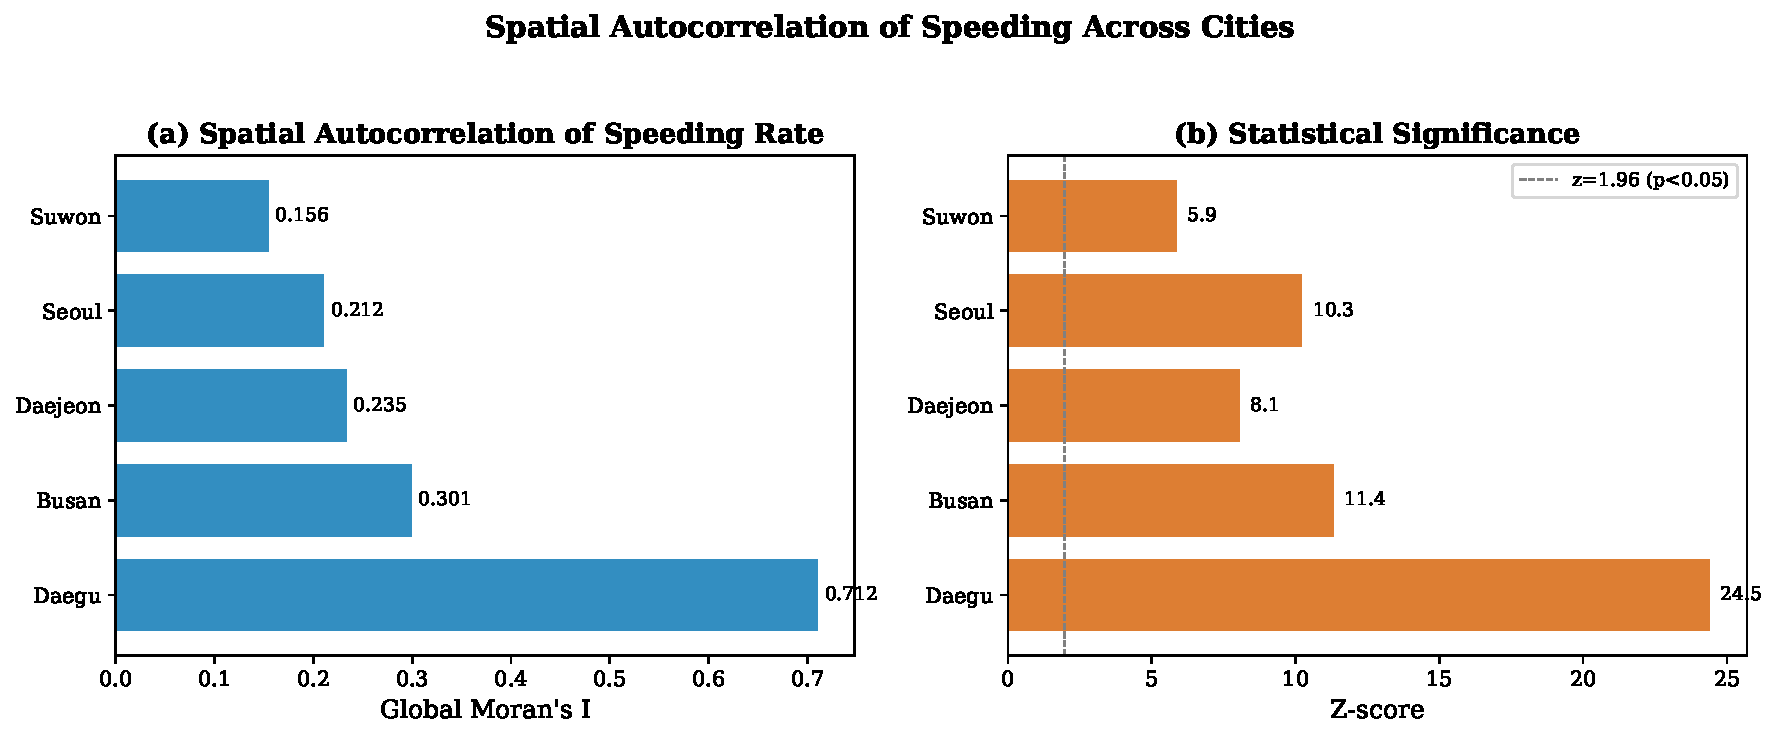
\includegraphics[width=0.85\textwidth]{fig_morans_comparison.pdf}
\end{frame}

\begin{frame}{Backup: Infrastructure Overlay}
\centering
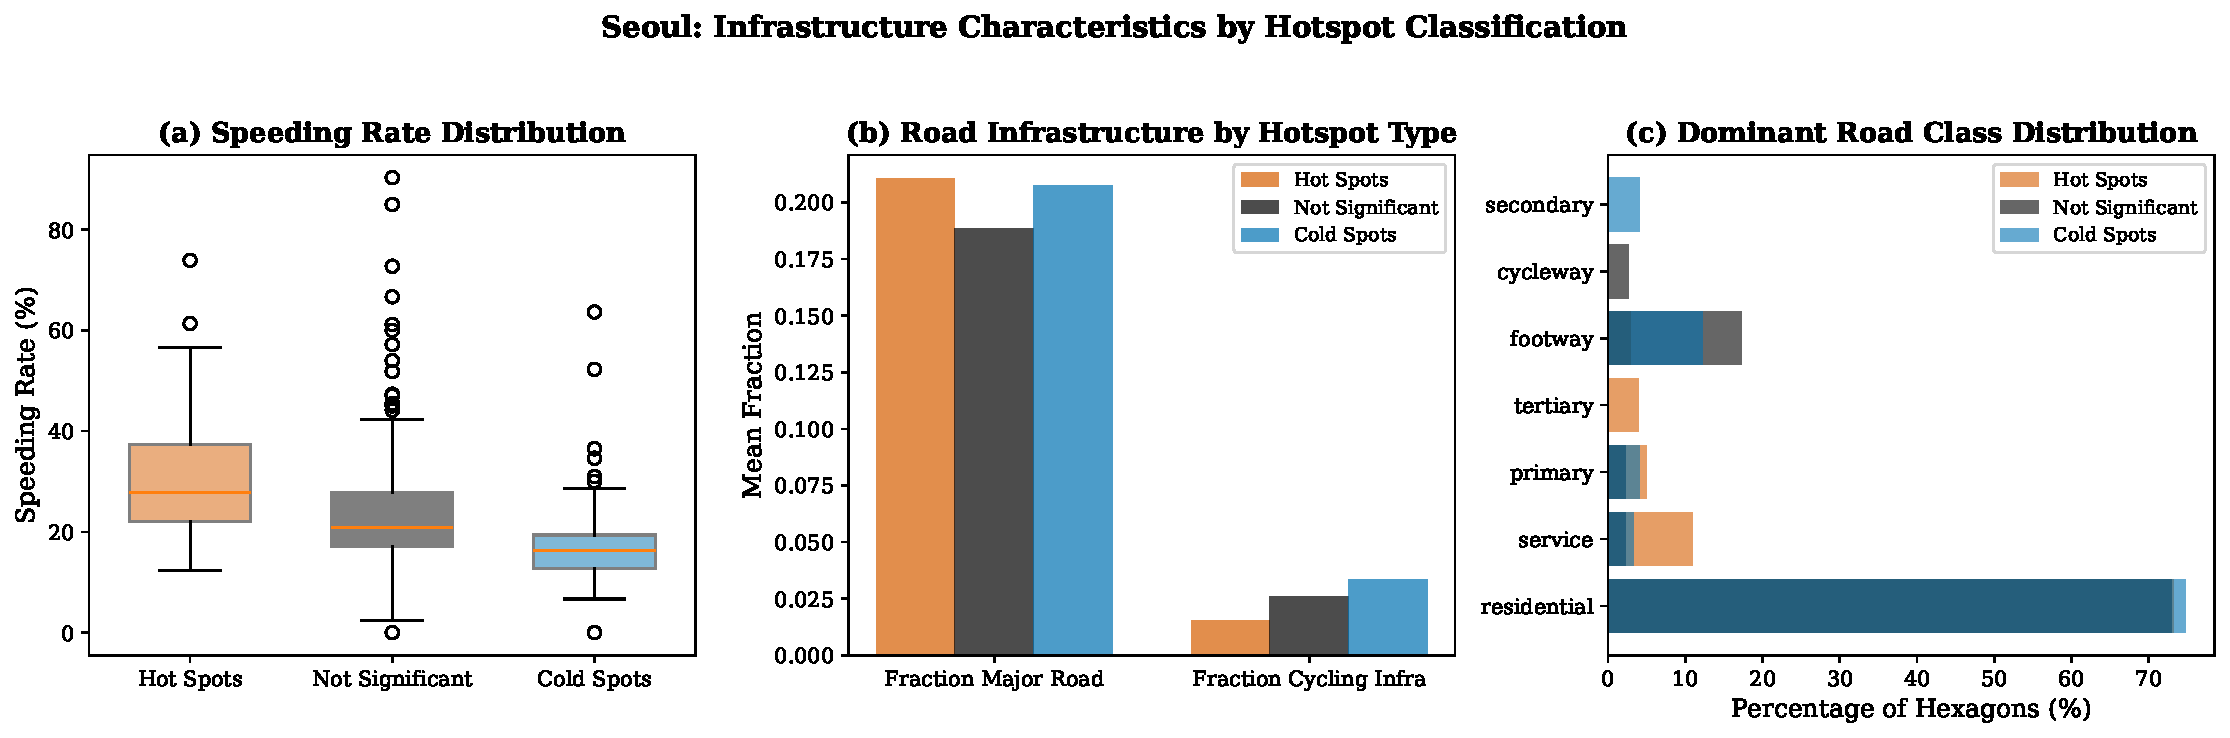
\includegraphics[width=0.85\textwidth]{fig_hotspot_infrastructure.pdf}
\end{frame}

\begin{frame}{Backup: DiD Robustness}
\begin{columns}
\begin{column}{0.48\textwidth}
\centering
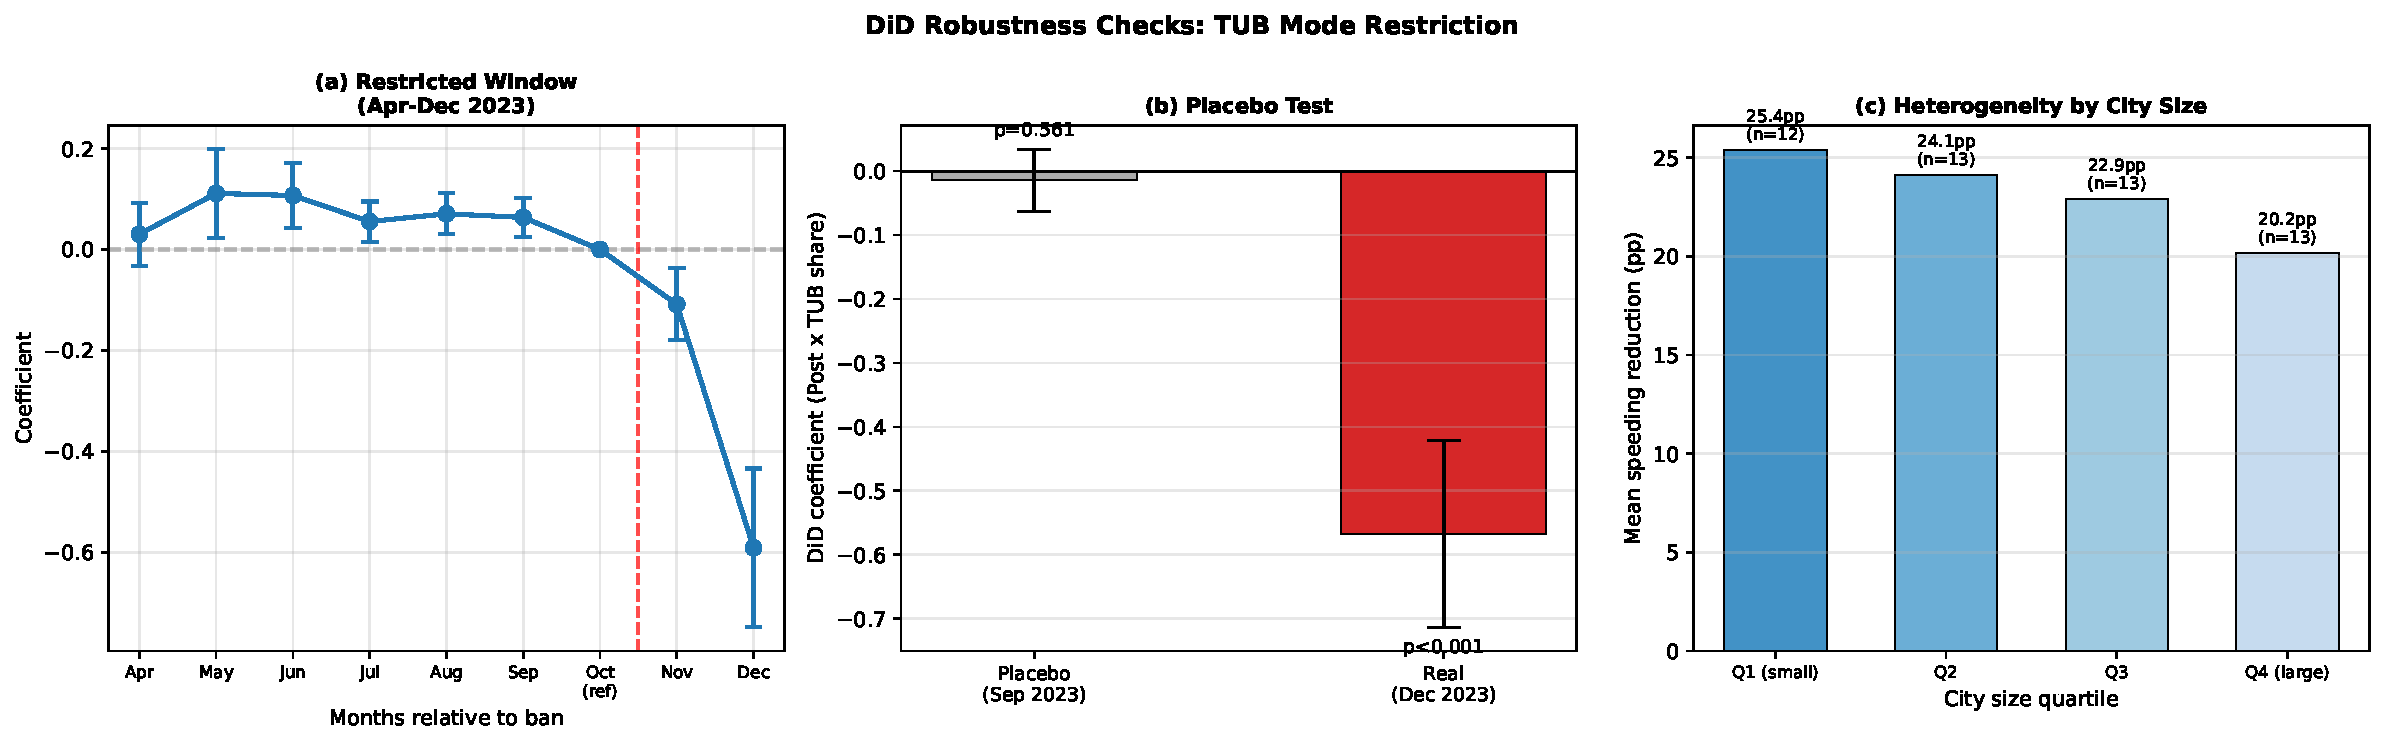
\includegraphics[width=\textwidth]{fig_did_robustness.pdf}
\end{column}
\begin{column}{0.48\textwidth}
\centering
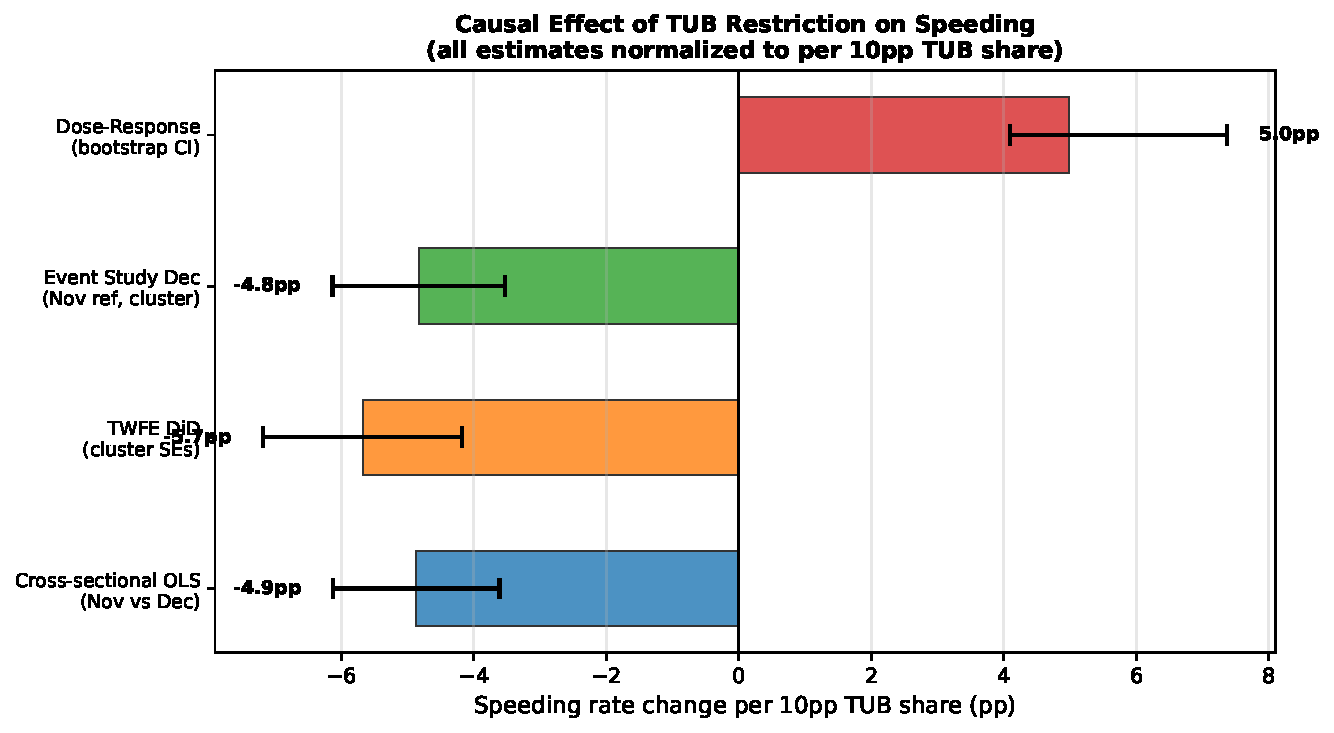
\includegraphics[width=\textwidth]{fig_did_summary_v2.pdf}
\end{column}
\end{columns}
\end{frame}

\begin{frame}{Backup: Curvature Risk Paradox}
\begin{columns}
\begin{column}{0.48\textwidth}
\centering
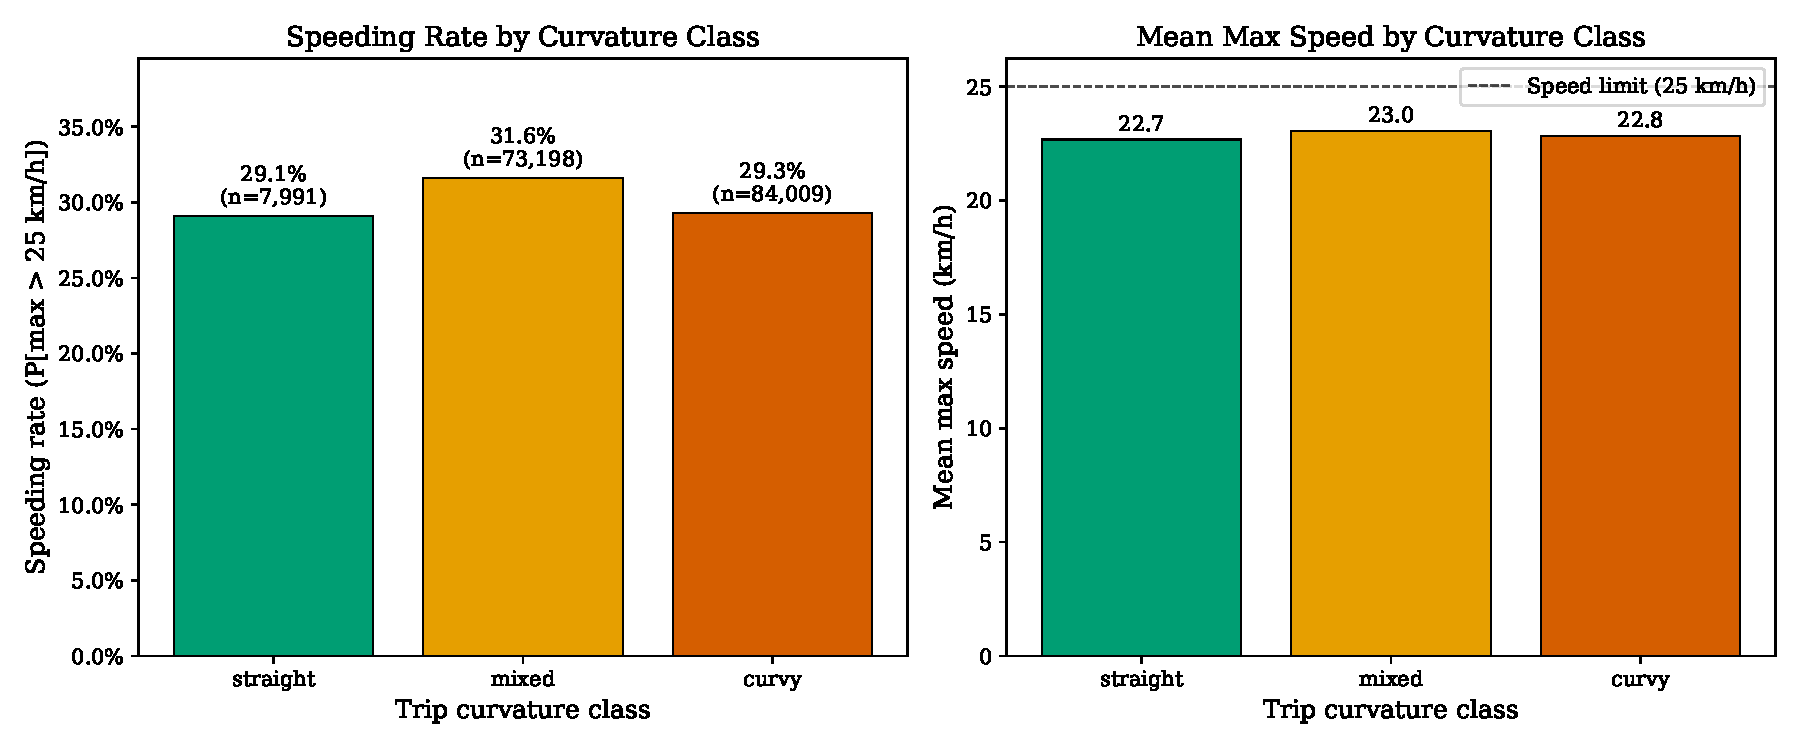
\includegraphics[width=\textwidth]{fig_curvature_speeding_rate.pdf}
\end{column}
\begin{column}{0.48\textwidth}
\centering
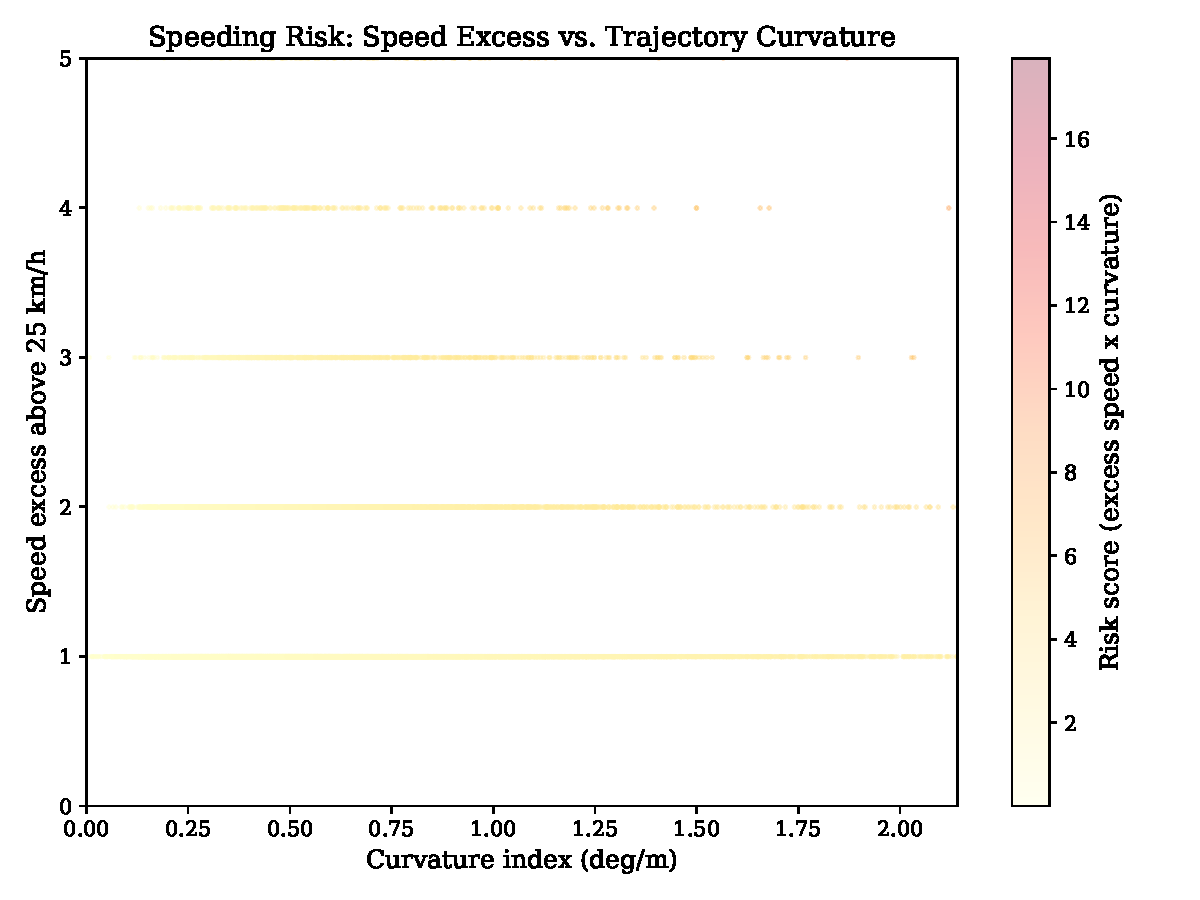
\includegraphics[width=\textwidth]{fig_curvature_risk_scatter.pdf}
\end{column}
\end{columns}
\end{frame}

\begin{frame}{Backup: Cox Proportional Hazards}
\centering
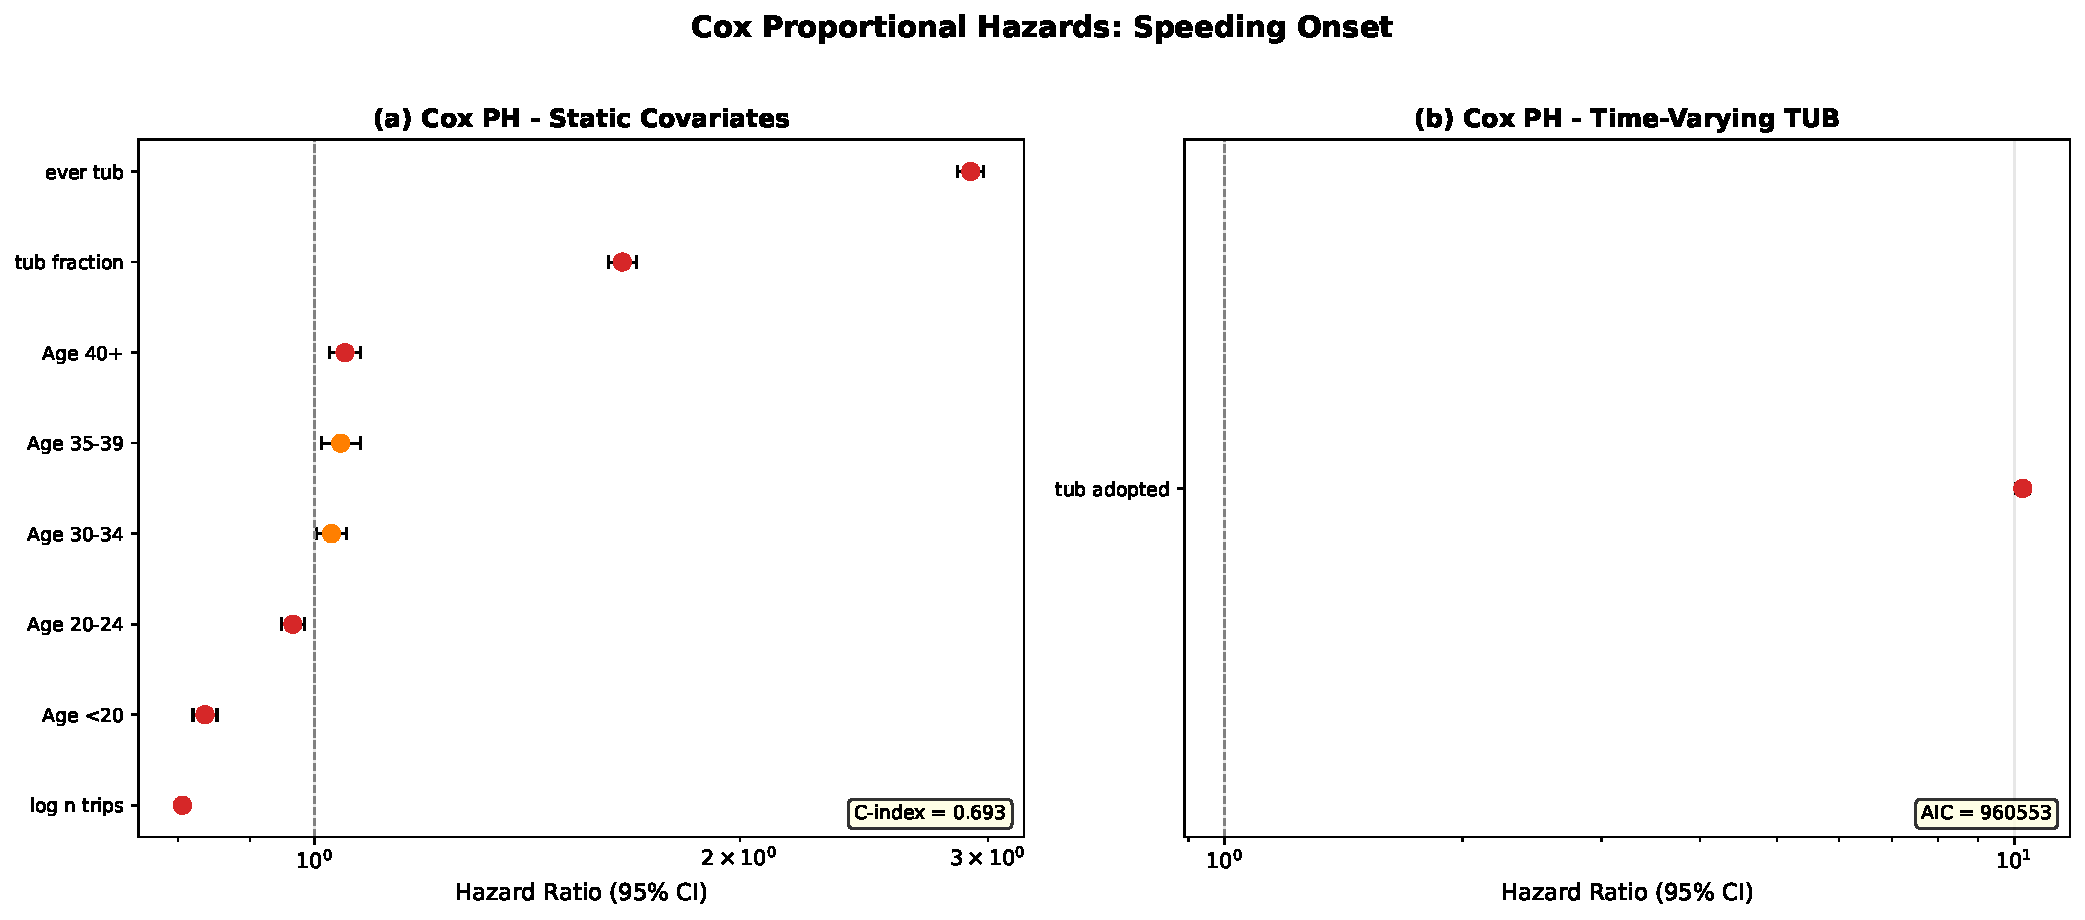
\includegraphics[width=0.85\textwidth]{fig_survival_cox.pdf}
\end{frame}

\end{document}
